\documentclass[aps,pra,superscriptaddress]{revtex4}
%\documentclass[aps,pra,superscriptaddress,showpacs]{revtex4}
\usepackage[intlimits]{amsmath}
\usepackage{amsfonts}
\usepackage{psfrag}
\usepackage{array}
%\usepackage[square]{natbib}
\usepackage{float}

%\usepackage{graphics}
\usepackage{subfigure}
\usepackage{enumitem}
\usepackage[usenames]{color}
%\usepackage{indentfirst}
\frenchspacing




\def\pdfshellescape{1}

\pdfadjustspacing=1

\hoffset=1.1truecm
\voffset=0.8in


\advance\voffset by -1cm
\advance\hoffset by -0.5cm
\textwidth=16cm
\textheight=23.5cm


\newcommand\be            {\begin{equation}}
\newcommand\bea           {\begin{equation}\begin{array}l\displaystyle}
\newcommand\ee            {\end{equation}}
\newcommand\bes           {\begin{subequations}}
\newcommand\esu           {\end{subequations}}
\newcommand\erf[1]        {\eqref{#1}}
\newcommand\labl[1]       {\label{#1}\ee}
\renewcommand{\(}{\left(}
\renewcommand{\)}{\right)}
\renewcommand{\[}{\left[}
\renewcommand{\]}{\right]}


%\renewcommand{\theenumi}{\Alph{enumi}}
\newcommand{\ud}{\mathrm d}

\newcommand{\bigx}[1]{\bBigg@{#1}}

\def\Bone{\hbox{1\!\!\!\!1}}
\newcommand\corr[1]       {\big\langle\,#1\,\big\rangle}
\newcommand\eps           {\varepsilon}
\newcommand\fii           {\varphi}
\newcommand\llangle       {\langle\!\langle}
\newcommand\mc            {\mathcal}
%\newcommand\ol            {\overline}
\newcommand\rrangle       {\rangle\!\rangle}

\newcommand\sg           {sinh--Gordon }
\newcommand\LL           {Lieb--Liniger }
\newcommand\p            {\partial}
\newcommand\psid         {\psi^{\dagger}}
\renewcommand\th         {\theta}
\newcommand\kb           {k_\text{B}}
\newcommand\ket[1]{|#1\rangle}
\newcommand\bra[1]{\langle #1 |}
\newcommand\braket[3]{\langle #1 | #2 | #3 \rangle }
\newcommand\tr {\mathrm{Tr}}
\newcommand\med[1]{\langle #1 \rangle }


\renewcommand\vec[1]{{\vert{#1}\rangle}}
\newcommand\vecc[1]{{\vert\hspace{1pt}#1\hspace{1pt}\rrangle}}
\newcommand\vvecc[1]{{\vert\hspace{-1pt}\vert\hspace{1pt}#1\hspace{1pt}\rrangle}}
\newcommand\cev[1]{{\langle{#1}\vert}}
\newcommand\ccevv[1]{{\langle\!\langle\hspace{1pt}#1\hspace{1pt}\vert\hspace{-1pt}\vert}}
\newcommand\vac{{\vec 0}}
\newcommand\cav{{\cev 0}}
\newcommand\vev[1]{{\langle#1\rangle}}
\newcommand\FF[1]{{\langle0\vert#1\vert\th_1,\dots,\th_n\rangle}}
\newcommand\no[1]{{\,:\!#1\!:\,}}
\def\ceev#1#2{{\langle{#1}\vert{#2}\rangle}}
\def\3pt#1#2#3{{\langle{#1}\vert{#2}\vert{#3}\rangle}}

\newcommand\arxiv[2]      {\href{http://arXiv.org/abs/#1}{#2}}
\newcommand\doi[2]        {\href{http://dx.doi.org/#1}{#2}}
\newcommand\httpurl[2]    {\href{#1}{#2}}
\newcommand{\EQ}{\begin{equation}}
\newcommand{\EN}{\end{equation}}
\usepackage{epsfig}
\usepackage{color}
\usepackage{psfrag}
%\usepackage{epstopdf}
\usepackage{amsmath}
\usepackage{graphicx}
\usepackage{amsfonts}
\usepackage{amssymb}
%\usepackage{epsfig}
\begin{document}
\bibliographystyle{plainnat}


\title{{\Large {\bf The Coprime Chain}}}

\author{G. Mussardo}
\affiliation{SISSA and INFN, Sezione di Trieste, via Bonomea 265, I-34136, 
Trieste, Italy}
\affiliation{International Centre for Theoretical Physics (ICTP), 
I-34151, Trieste, Italy}
%\affiliation{International Institute of Physics, Natal, Brasil} 
\author{G. Giudici}
\affiliation{SISSA and INFN, Sezione di Trieste, via Bonomea 265, I-34136, 
Trieste, Italy}
\author{J. Viti} 
\affiliation{ECT \& Instituto Internacional de Fisica, UFRN, Lagoa Nova 59078-970 Natal, BrazilUFRN}

\begin{abstract}
\noindent

In this paper we introduce and study the $q$-coprime chain, i.e. a strongly correlated quantum system defined in terms of 
the integer eigenvalues $n_i$ of the occupation number operators of each site of a chain of length $M$. The $n_i$'s take value  
in the interval $(2,q)$ and may be regarded as $S_z$ values in spin representation $j = \frac{q-2}{2}$. 
The distinguished interaction of this model is based on the coprimality matrix $\widehat \Phi$ which, for the ferromagnetic case, 
assigns lower energy to neighbor sites with occupation numbers $n_i$ and $n_{i+1}$ that have a common natural divisor, while 
for the anti-ferromagnetic case, to neighbor sites whose occupation numbers $n_i$ and $n_{i+1}$ are coprime numbers. 
The $q$-coprime chain, both in the ferro and anti-ferro magnetic cases, may have an exponential number of ground states 
ruled by the adjacency matrix of the ground states.




\vspace{3mm}
\noindent
Pacs numbers: 11.10.St, 11.15.Kc, 11.30.Pb

\end{abstract}
\maketitle



\section{Introduction}
\label{sec:intro}
\noindent

Discrete vs continuous mathematics; 

prime numbers; 

primality; 

exponential degeneracy of the vacua; 

Presence of gap 

Classical statistical model: absence of phase transition, only disorder phase 

lift of the degeneracy 

strongly correlated systems; 

quench processes 

coprime model: ferro and antiferromagnet, generalization of the Potts model 

Graph theory 


\section{Definition of the model}
\label{sec:def}
\noindent
In this section we are going to introduce the coprime model and its general quantum Hamiltonian for the case of a one-dimensional chain made of 
$M$ sites. 

\vspace{3mm}
\noindent
{\bf Hilbert Space}. The coprime model involves the dynamics of the occupation number operators $N_i$ at each site $i$ of the chain. Such operators 
are characterised by their eigenvalues which take $(q-1)$ integer values in the range  
\be
n_i \,=\,2,3,\ldots q \,\,\,.
\label{possiblevalues}
\ee 
For reasons that become clear soon, we have shifted the usual values of the occupation number by $2$, so that the lowest possible value of each occupation number is $2$ while the maximum is $q$. We assume that the gas described by these occupation numbers obeys a bosonic statistics, although 
there is a cut-off to the higher value of their occupation numbers. For such a system we can also define at each site the annihilation and creation operators $c_i^-$ and $c_i^+ = (c_i^-)^\dagger$, with the properties  
\be 
c_i^-\,\mid 2 \rangle \,=\, 0 
\hspace{5mm}
,
\hspace{5mm}
c_i^+ \, \mid q \rangle \,=\, 0 
\,\,\,\,\,\,\,\,\,\,\,\,\,
,
\,\,\,\,\,\,\,\,\,\,\,\,\,
\forall i \,\,\,.
\ee
The simplest way to look at the quantum occupation numbers of this boson system is to regard the $(q-1)$ values of the $N_i$ operators 
as the eigenvalues of the $S_z$ component of an ordinary spin in representation $j = \frac{q-2}{2}$: in order to match the eigenvalues 
$m$ of $S_z$ with the values (\ref{possiblevalues}), we can use in this case the relationship
\be 
m \,=\, n_i -\frac{q+2}{2} \,\,\,. 
\ee
Using this mapping of the occupation number operators onto a spin system, we can then define the action of $c_i$ and $c_i^\dagger$ 
on each state as  
\be 
\begin{array}{l}
c_i^- \,\mid n_i \rangle \,=\,\sqrt{(n_i -2) \,(q - n_i +1)} \,\mid n_i -1\rangle \\
\\
c_i^+ \,\mid n_i \rangle \,=\, \sqrt{(q - n_i) (n_i -1)} \,\,\,\,\mid n_i +1 \rangle 
\end{array}
\ee
These operators satisfy the commutation relations 
\begin{eqnarray}
\left[N_i , c_i^\pm \right] &\,=\,&  \pm \, c_i^\pm  \label{commutationrelation}\\
\left[c_i^+ , c_i^-\right] & \,=\, & N_i - \frac{(q-2)}{2}   
\end{eqnarray}
Hence, on a chain of $M$ sites, the dimension of the Hilbert space is ${\rm dim}\, {\cal H} = (q-1)^M$ and its Fock space is spanned by the 
vectors 
\be 
\mid n_1, n_2, \ldots n_M \rangle \,=\, \mid n_1 \rangle \, \otimes \,\mid n_2 \rangle \, \cdots \,\otimes \, \mid n_M \rangle \,\,\,
\ee
which are identified by the occupation number at each site of the chain. A typical configuration of the coprime model is shown in Figure \ref{coprimechainmodel}. 

\begin{figure}[t]
\begin{center}
%\vspace{8mm}
\psfig{figure=Figures/Coprimechainmodel.jpg,height=5cm,width=8cm}
\caption{{\em A configuration of the coprime model relative to $q=6$.}}
\label{coprimechainmodel}
\end{center}
\end{figure}

In the following we will consider various boundary conditions for such a chain, 
such as periodic and fixed boundary conditions, the former associated to the condition $n_{i+M} \,=\,n_i$, the latter to two fixed values of both $n_1$ and $n_M$. 

\vspace{3mm}
\noindent
{\bf Quantum Hamiltonian}. 
In order to introduce the quantum Hamiltonian of our model, it is first convenient to consider the arithmetic function 
\be \label{coprimalityfunction}
\Phi(a,b) \,=\,
\left\{ 
\begin{array} {lll}
0 & & {\rm if} \, {\rm gcd}(a,b) =1 \\
1 & & {\rm if} \, {\rm gcd}(a,b) \neq 1 
\end{array}
\hspace{5mm}
,
\hspace{5mm}
a,b \in \mathbb{N}
\right. 
\ee
where ${\rm gcd}(a,b)$ stays for the greatest common divisor between the two natural numbers $a$ and $b$. In the following we will say that 
two integers $a$ and $b$ are coprime if their greatest common divisor is just $1$.  We call $\Phi(a,b)$ the {\em coprimality function} and we will discuss in more detail its properties in Section \ref{coprimality}. 

\vspace{1mm}
As a general form of the quantum Hamiltonian of our model we will take   
%\be 
%H \,=\,-\sum_{i=1}^M \Phi(n_i,n_{i+1}) - J \,\sum_{i=1}^M (c_i^\dagger \,c_{i+1} + c_{i+1}^\dagger\,c_i) -
%\sum_{i=1,\alpha}^M \lambda_{\alpha} B^{\alpha}_i  
%\ee
\be 
H \,=\,-\sum_{i=1}^M \left[\Phi(n_i,n_{i+1}) + J  (c_i^+ \,c_{i+1}^- + c_{i+1}^+ \,c_i^-) + 
\sum_{\alpha=1}^{(q-1)^2} \lambda_{\alpha} B^{\alpha}_i   + h \,\delta(s,n_i)\right] \,\,\,. 
\label{quantumhamiltonian}
\ee
Let's stress that the fingerprint of our coprime model is the omnipresence of the term $\Phi(n_i,n_{i+1})$ in its Hamiltonian: it is for this reason that this term has its coupling constant equal to 1 and therefore can never be switched to zero. Notice that this interaction term makes the model qualitatively different from any other more familiar spin chain model considered in the literature. As a last comment, as it is written the quantum Hamiltonian above refers to the 
{\em ferromagnetic case}, since it privileges equal (and common divisible) values of the occupation numbers of neighbor sites: the {\em antiferromagnetic case} can be easily obtained by changing in the Hamiltonian above 
\be 
\Phi(a,b) \rightarrow 1 - \Phi(a,b)\,\,\,. 
\label{antiferromagnetic}
\ee
With this transformation we make more favourable configurations in which two nearby sites have different occupation numbers or 
without any common divisors. Let's now discuss the meaning of the other couplings. 

The coupling constant $J$ is of course responsabile for the hopping process of destroying a boson at the site $i$ and creating it at the neighbor site $i+1$ (and viceversa) 
\be
\begin{array}{l}
c_i^+ c_{i+1}^- \,\mid n_i \rangle \,\otimes \,\mid n_{i+1}\rangle \,=\, \sqrt{(q - n_i) (n_i -1)(n_{i+1} -2) \,(q - n_{i+1} +1)} \, 
\mid n_i + 1 \rangle \,\otimes \,\mid n_{i+1} -1 \rangle \\
\\
c_{i+1}^+ c_{i}^- \,\mid n_i \rangle \,\otimes \,\mid n_{i+1}\rangle \,=\, \sqrt{(q - n_{i+1}) (n_{i+1} -1) (n_{i} -2) \,(q - n_{i} +1)} \, 
\mid n_i - 1 \rangle \,\otimes \,\mid n_{i+1} +1 \rangle
\end{array}
\ee 
The operators $B_i^{\alpha}$ have the local form 
\be 
B_i^{\alpha} \,=\, {\bf 1} \otimes {\bf 1} \cdots {\bf 1} \otimes \underset{\underset{i-site}{\uparrow}}{{\mathcal B}^{\alpha}} \otimes {\bf 1} \otimes {\bf 1} \cdots \otimes {\bf 1}  
\ee
where ${\mathcal B}^{\alpha}$, with $\alpha=1,2,\ldots (q-1)^2$, is one of the $(q-1)^2$ possible hermitian matrices acting on the $(q-1)$ dimensional 
Hilbert space at the site $i$ while ${\bf 1}$ is the $(q-1)\times (q-1)$ identity matrix acting on each of the remaining sites. We will see later 
how the various phases and ground states of the model change by switching on different operators ${\mathcal B}_i^\alpha$ and how, using 
some combination of them, we can filter particular phases of the model. Finally, the coupling constant $h$ in eq.(\ref{quantumhamiltonian}) is a global magnetic field that polarises the occupation numbers $n_i$ along an assigned value $s$. 

The structure of the vacua of the coprime model, in particular their nature and how they vary by moving the various couplings present in the quantum Hamiltonian (\ref{quantumhamiltonian}) will the subject of the next Sections of this paper. It is worth stressing that, apart from some trivial limits (as for instance sending $h \rightarrow \infty$), the coprime model seems to be genuinely a non-integral model.   

%Let's now move to discuss in more detail instead the nature of the coprimality matrix associated to the arithmetic function $\Phi(a,b)$.  

\section{The Coprimality matrix}\label{coprimality}
\noindent

\vspace{3mm}
\noindent
{\bf Basic Arithmetic}. 
Before starting the discussion on the coprimality function $\Phi(a,b)$, let's recall that a basic result of number theory is the unique decomposition of 
a natural number $n$ into its prime factors $p_i$, together with their relative multiplicities $\sigma_i$ 
\be 
n \, =\, p_1^{\sigma_1} \, p_2^{\sigma_2} \, \cdots p_l^{\sigma_l} 
\label{primedecomposition}
\,\,\,.
\ee
Simple as it is, this observation will turn out to be useful pretty soon. Moreover, it is also useful to recall two simple related properties of the prime numbers: 
the first is that, for any integer $n$, there is always a prime $p$ in the interval $(n, 2n)$, alias 
\be 
n < p < 2n \,\,\,,
\label{doppio}
\ee 
The second rule, somehow equivalent to the previous one, concerns a bound on the $(k+1)$-th prime number in terms of $p_k$
\be
p_{k+1} < 2 \,p_k \,\,\,.
\label{twiceprime}
\ee
Finally, let's remember the approximate formula for the $n$-th prime number 
\be 
p_n \sim n \, \log n\,\,\,.
\label{approximateprime}
\ee
 
\vspace{3mm}
\noindent
{\bf Coprimality}. 
Let's now turn our attention to the coprimality function: once we fix the maximum value $q$ assumed by the number operators $N_i$, 
we can define the $(q-1) \times (q-1)$ {\em coprimality matrix} $\widehat\Phi$ whose matrix elements are expressed by the coprimality function $\Phi(a,b)$
\be 
\langle a \mid \widehat\Phi \mid b \rangle \,=\, \Phi(a,b) \,\,\,.
\label{coprimalitymatrix}
\ee
$\widehat\Phi$ is then a real symmetric matrix made of $0$ and $1$ with some peculiar properties which can be recovered by well known results in number theory. First of all, given its definition, it is easy to see that the matrix element $\Phi(a,b)$ is testing whether or not the two integer numbers $a$ and $b$ have some common divisor greater than $1$: hence, it gives as output $1$ when they share some common divisor, otherwise $0$ if they are coprime. For the peculiar role played by the integer number $1$, which acts as a "neutral" divisor of all natural numbers, it seems wise to exclude it from the list of possible values assumed by the occupation numbers and therefore to start from the value $2$, as we actually do, so that there is not, a priori, any privileged value among the entire set of occupation numbers. Hence, what $\Phi(a,b)$ is checking is then a looser property than just the strict primality of the two individual numbers $a$ and $b$: so, if $a$ and $b$ were both primes, say $a = 3$ and $b=11$, obviously $\Phi(3,11) =0$ but one could also get $0$ when the two numbers are instead composite, since it is enough that they do not have any common divisor as it happens, for instance, choosing $a = 30 = 2 \times 3\times 5$ and $b = 77 = 7 \times 11$. In other words, the coprimality matrix $\widehat\Phi$ is sensitive to the {\em multiplicative} structure of the natural numbers rather than their {\em additive structure}. Notice that, with our definition of $\widehat\Phi$, all its diagonal elements are equal to $1$, so that ${\rm Tr}\, \widehat\Phi = (q-1) $. 

\vspace{3mm}
\noindent
{\bf Prime-Number Vectors}. Given the multiplicative nature of the function $\Phi(a,b)$ it is useful to introduce an alternative representation 
for the $(q-1)$ numbers involved in the coprimality matrix $\widehat\Phi$. The first step to do so is to identify the set of the $l$ prime numbers less than $q$ which, therefore, are among the allowed values (\ref{possiblevalues})
\be
{\mathcal P} \,=\,\{2,3,5,\ldots p_{l-1}, p_l\}  
\hspace{5mm}
,
\hspace{5mm} p_l \leq q \,\,\,. 
\ee
The total number $l$ of these primes -- as a function of $q$ -- is given by the prime-counting function $\pi(q)$ which, for our present purposes, 
can be approximated by the {\em integral logarithm function} ${\rm Li}(q)$ given by 
\be
\pi(q) \simeq \int_2^q \frac{dt}{\log(t)} \equiv {\rm Li}(q)\,\,\,.
\label{countingprime}
\ee
Since ${\rm Li}(x) \simeq x/\log(x)$, the number of primes present in the interval $(2,q)$ is thus roughly $l \simeq q/\log q$.  
This estimate tells us that there is always a sufficient number of primes in each interval $(2,q)$ of the possible values of the occupation number, although their number is (logarithimically) smaller than $q$ itself. 

Consider now a series of $l$-dimensional boolean vectors (which we called {\em prime number vectors}) associated to $l$ boxes in 
correspondence to the primes in the interval $(2,q)$ as 
\begin{figure}[h!]
\begin{center}
%\vspace{8mm}
\psfig{figure=Figures/PrimeBox.jpg,height=5cm,width=6cm}
%\caption{{\em Density of zeros versus the dimension $q$ of the coprimality matrix $\widehat\Phi$. The red line 
%shows the theoretical value $\rho_0 \simeq 0.3920...$}}
\label{boxes}
\end{center}
\end{figure}

Using the prime decomposition (\ref{primedecomposition}) of each natural number $n$ in terms of the primes, we can associate to each number $n$ in the interval $ (2,q)$ a prime-number vector simply obtained by filling the $k$-th box with $1$ if the prime $p_k$ is present in the prime decomposition of $n$ (independently of its multiplicity), or putting $0$ otherwise. In other words, with this association we "flatten" the various powers $\sigma_n$ of the prime number decomposition (\ref{primedecomposition}) of $n$, namely we just keep track of the information whether the prime $p_k$ is present or not in the decomposition of the natural number $n$. So, for instance, imagine to have $q = 37$: in this case the ${\mathcal P}$ has cardinality $l = 12$ and this set consists of the prime numbers 
$$
{\mathcal P} = \{2, 3, 5, 7, 11, 13, 17, 19, 23, 29, 31, 37\} \,\,\,.
$$
In this case we have then a $12$-dimensional prime-number vector space and, for example, with the rule given above the number $36$ will be represented in terms of the prime-number vector as 
$$ 
n = 36 = 2^2 \,\times\, 3^2 \,\,\,\longrightarrow \,\,\,(1,1,0,0,0,0,0,0,0,0,0,0) \,\,\,.
$$
Since the dimension of the prime-number vector space is smaller than $q$, and moreover not all $l$-dimensional boolean vectors are present in 
the prime-number vector space \footnote{It is obvious, for instance, that the vector $y = (1,1,1,\ldots, 1,1,1)$ made of all $1$'s cannot 
be in the prime-number space, because it would correspond, at least, to the natural number $n = p_1 p_2 \ldots p_l$ (i.e. to the number given by the 
product of all the $l$ primes) which is much great than the maximum number $q$ of the interval. Similar consideration may be applied to other 
boolean $l$-dimensional vectors.}, these two facts taken together imply that there will be a certain degree of degeneracy in this mapping, i.e. different integers will be associated to the same prime number vector. In other words, all the integers in the interval $(2,q)$ will fall into different {\em classes of equivalence} which are identified by the their prime-number vectors. For instance, all numbers that are pure powers of $2$ will belong to the same class of equivalence associated to the same $l$-dimensional vector $v = (1,0,0,0,0,\ldots, 0)$, as well as all the pure powers of $3$ belong to another class of equivalence associated to the $l$-dimensional vector $w = (0,1,0,0,0,\ldots,0)$.   

In summary, with the procedure described above, we can then associate to each natural number $n$ its class of equivalence and its  
prime number representative vector $v_n$ 
\be 
n = 2^{\sigma_2} \, \cdot\, 3^{\sigma_3} \ldots p_k^{\sigma_k} \cdot \, p_s^{\sigma_s} \,\,\,
\longrightarrow \,\,\, v_n \,=\, (1, 1, \ldots 
\underset{\underset{k}{\uparrow}}{1}, 0, \ldots, 0, \underset{\underset{s}{\uparrow}}{1}\ldots, 0) \,\,\,.
\ee
To make an explicit example, for $q=37$ we have the following $23$ classes of equivalence 
\be
\begin{array}{llll}
(2,4,8,16,32) & & \rightarrow & (1,0,0,0,0,0,0,0,0,0,0,0) \\
(3,9,27) & &\rightarrow & (0,1,0,0,0,0,0,0,0,0,0,0) \\
(5,25) & &\rightarrow & (0,0,1,0,0,0,0,0,0,0,0,0) \\
(6,12,18,24,36) & & \rightarrow & (1,1,0,0,0,0,0,0,0,0,0,0) \\
(7) & & \rightarrow & (0,0,0,1,0,0,0,0,0,0,0,0) \\
(10,20) & & \rightarrow  & (1,0,1,0,0,0,0,0,0,0,0,0) \\
(11) & & \rightarrow &  (0,0,0,0,1,0,0,0,0,0,0,0) \\
(13) & & \rightarrow & (0,0,0,0,0,1,0,0,0,0,0,0) \\
(14,28) && \rightarrow & (1,0,0,1,0,0,0,0,0,0,0,0) \\
(15) & &\rightarrow &  (0,1,1,0,0,0,0,0,0,0,0,0) \\
(17) & &\rightarrow &  (0,0,0,0,0,0,1,0,0,0,0,0) \\
(19) & & \rightarrow &  (0,0,0,0,0,0,0,1,0,0,0,0) \\
(21) & & \rightarrow &  (0,1,0,1,0,0,0,0,0,0,0,0) \\
(22) & & \rightarrow &  (1,0,0,0,1,0,0,0,0,0,0,0) \\
(23) & &\rightarrow &  (0,0,0,0,0,0,0,0,1,0,0,0) \\
(26) & & \rightarrow &  (1,0,0,0,0,1,0,0,0,0,0,0) \\
(29) & & \rightarrow &  (0,0,0,0,0,0,0,0,0,1,0,0) \\
(30) & & \rightarrow &  (1,1,1,0,0,0,0,0,0,0,0,0) \\
(31) & &\rightarrow &  (0,0,0,0,0,0,0,0,0,0,1,0) \\
(33) & & \rightarrow &  (0,1,0,0,1,0,0,0,0,0,0,0) \\
(34) & & \rightarrow &  (1,0,0,0,0,0,1,0,0,0,0,0) \\
(35) & &\rightarrow &  (0,0,1,1,0,0,0,0,0,0,0,0) \\
(37) & & \rightarrow &  (0,0,0,0,0,0,0,0,0,0,0,1) 
\end{array}
\ee
It is easy to see that one can give an easy lower bound to the number of classes of equivalence for large values of $q$: if we call this number ${\mathcal C}(q)$, for $q \gg 1$, we have 
\be
{\mathcal C}(q) >  \frac{3}{2} \frac{q}{\log q} \,\,\,. 
\label{lowerbound}
\ee
To show this, notice that there will be at least the $q/\log q$ classes of universality associated to the pure prime numbers $(p_1,p_2,\ldots, p_l)$ present in the interval $(0,q)$, to which we can add the classes of equivalence associated to the composite numbers $n_i = 2 \times p_i $ $ (i=1,2,\ldots ,s)$, 
with $p_s < q/2$. The number of these classes of equivalence is roughly equal to $\frac{q}{2 \log q/2} \simeq \frac{q}{2 \log q}$ which, 
added to $q/\log q$, produces the lower bound (\ref{lowerbound}). A "numerical experimental" determination of the classes of equivalence vs $q$ 
is shown in Figure \ref{numberclasses} where one can see a pronounced linear behavior in $q$, whose best fit gives the result 
\be 
{\mathcal C}(q) \simeq 
0.607591 \, q + 0.581306 \,\,\,, . 
\label{bestfitclasses}
\ee
 

\begin{figure}[t]
\vspace{8mm}
\psfig{figure=Figures/NumberClasses.pdf,height=6cm,width=10cm}
\caption{{\em Number of classes of equivalence versus $q$ of the coprimality model. 
matrix $\widehat\Phi$.}}
\label{numberclasses}
\end{figure}



For the nature of the interaction dictated by the coprimality matrix, it is easy to see that all vectors belonging to the same class of equivalence behave the same way. Moreover, the coprimality matrix itself can be expressed in terms of the matrix of the scalar product, alias the overlapping, of these prime-number vectors, since we have  
\be 
\phi(a,b) \,=\,\frac{\langle v_a \mid v_b \rangle}{d_{ab}} \,\,\,, 
\label{Gram}
\ee
where $d_{ab}$ is the total number of common divisors of the two numbers $a$ and $b$. Notice that the scalar product of coprime numbers 
simply vanishes. 
\begin{figure}[b]
\vspace{8mm}
\psfig{figure=Figures/ratio.eps,height=6cm,width=8cm}
\caption{{\em Density of zeros versus the dimension $q$ of the coprimality matrix $\widehat\Phi$. The red line 
shows the theoretical value $\rho_0 \simeq 0.3920...$}}
\label{ratiozeros}
\end{figure}

\vspace{3mm}
\noindent
{\bf Random Nature of the Coprimality Matrix}. 
The sensitivity to the multiplicative nature of the natural numbers awards to the matrix $\widehat\Phi$ a certain degree of randomness because, assuming that the matrix element $\phi(a,b)$ was know, it is impossible to predict just on this information the neighbor matrix element $\phi(a,b+1)$: passing from $b$ to $b+1$, we are in fact using the additive nature of the natural numbers, while $\phi(a,b)$ is just sensitive to their multiplicative nature. So, it can easily happen that adding $1$ to the number $b$ we can pass from a very highly compositive number to a prime number and viceversa: take for instance the highly compositive number $b = 2310 = 2 \times 3 \times 5 \times 7 \times 11$ and its consecutive number $b+1 = 2311$ which is instead a prime number. So, spanning all the values along each row of the matrix, we have essentially a random sequence of $0$ and $1$, whose average however can be predicted with a reasonable accuracy with a simple argument. 

We have in fact to relay on the loose correlations that exist among the primes, so that the the probability that a given integer $a$ is divisible by the prime $p_i$ is $1/p_i$ (since in any sequence of natural numbers, one out of $p_i$ is divisible for $p_i$) and the compositive probability that another number $b$ is also divisible for $p_i$ is then $1/p_i^2$. Therefore the probability that both $a$ and $b$ are not divisible by the same set of primes $p_i$ (making the broad assumption of independence among the primes) is then 
\be 
P \simeq \prod_{i=1} \left(1 - \frac{1}{p_i^2}\right) \,=\,\frac{1}{\zeta(2)} \,=\,\frac{6}{\pi^2} = 0.607927 \,\,\,.
\ee
where $\zeta(s)$ is the Riemann function. Given that $(q-1)^2$ is the total number of elements present in the 
matrix $\widehat\Phi$, this brings to the following estimates of the densities $\rho_0$ and $\rho_1$ 
of $0$'s and $1$'s in the coprimality matrix 
\be
\rho_0 \,=\,\frac{N_0}{(q-1)^2} \simeq  0.607927 
\hspace{5mm}
, 
\hspace{5mm}
\rho_1 \,=\,\frac{N_1}{(q-1)^2} \simeq (1-P) = 0.392073 \,\,\,, 
\ee
where $N_{0}$ and $N_1$ are the total numbers of $0$'s and $1$'s in $\widehat\Phi$. These predictions can be easily tested by performing "numerical experiments" on the matrix $\widehat\Phi$ by varying its dimensionality: some of the values which were got doing these computations are shown in the Table 1,while the more extensive set of values are shown in Figure \ref{ratiozeros}. As one can see, the agreement is reasonably good, of the order of few percents.     


\begin{table}[b]\label{pifre}
\begin{center}
\begin{tabular}{|l|l|l|} \hline 
$q$ & Numbers of $0$'s & Estimate of $\rho_0$ \\
\hline \hline
$100 $ & \,\,\,\,\,\,\,\,\,\,\,$3913$ &  \,\,\,\,\,\,\,\,$ 0.399245$ \\
$ 150$ & \,\,\,\,\,\,\,\,\,\,\,$ 8785$ &  \,\,\,\,\,\,\,\,$ 0.395703$ \\
$ 200$ & \,\,\,\,\,\,\,\,\,\,\,$ 15537$ &  \,\,\,\,\,\,\,\,$0.392339 $ \\
$ 250$ & \,\,\,\,\,\,\,\,\,\,\,$24453 $ &  \,\,\,\,\,\,\,\,$0.394397$ \\
$ 300$ & \,\,\,\,\,\,\,\,\,\,\,$ 32205$ &  \,\,\,\,\,\,\,\,$0.393788 $ \\
$ 350$ & \,\,\,\,\,\,\,\,\,\,\,$ 47841$ &  \,\,\,\,\,\,\,\,$ 0.39279$ \\
$ 400$ & \,\,\,\,\,\,\,\,\,\,\,$ 62645$ &  \,\,\,\,\,\,\,\,$0.393496 $ \\
$ 450$ & \,\,\,\,\,\,\,\,\,\,\,$79233 $ &  \,\,\,\,\,\,\,\,$0.393019$ \\
$ 500$ & \,\,\,\,\,\,\,\,\,\,\,$ 97769$ &  \,\,\,\,\,\,\,\,$0.392645 $ \\
\hline 
\end{tabular} 
\end{center}
Table 1. Series of trials in order to test the goodness of the theoretical estimate of the total number of $0$'s present in the 
coprimality matrix $\widehat\Phi$. 
\end{table}
\vspace{1mm}

\begin{figure}[t]
%\vspace{8mm}
\psfig{figure=Figures/Comparison.jpg,height=12.5cm,width=17cm}
\caption{{\em (a): Graphical representation of the coprimality matrix $\widehat\Phi$ in comparison to (b) a similar representation of a random 
matrix with the same density of $0$'s.}}
\label{comparison}
\end{figure}



\vspace{3mm}
\noindent
{\bf Graphical Representation and Fourier Transform}. 
It is interesting to associate to the pair of natural numbers $(a,b)$ a point in a two dimensional plane: in this way, we cover the first quadrant of the cartesian plane in terms of an integer lattice points. Notice that the two integers $a$ and $b$ are coprime if and only if the point with coordinates (a, b) in the Cartesian coordinate system is "visible" from the origin (0,0), in the sense that there is no point with integer coordinates on the line segment between the origin and the point of coordinates $(a, b)$. 


\begin{figure}[t]
%\vspace{8mm}
\psfig{figure=Figures/Fourier.jpg,height=12.5cm,width=17cm}
\caption{{\em  Absolute module of the Discrete Fourier Transform of (a) the coprimality matrix $\widehat\Phi$ and (b) in comparison to (b) of a random 
matrix with the same density of $0$'s. For both the matrices, the dimensionality is $q=200$.}}
\label{Fourier}
\end{figure}


This cartesian picture suggests a graphical representation of the coprimality matrix, obtained by associating a black pixel to the $1$'s and a white pixel to the $0$'s: this is shown in Figure \ref{comparison}, also in comparison with a similar picture for a random matrix made of $0$ and $1$ which has the same density $\rho_0$ of the coprimality matrix and all 1 along the main diagonal. By looking at these two pictures, one can see that there is a certain degree of "order" in the coprimality matrix -- order that seems to be on the contrary absent in the genuine random matrix with the same density of $0$'s. For spell out in more detail the texture of the coprimality matrix, assume first that we have extended it to arbitrarily large values of $q$: in this case observe that its matrix elements satisfy the following properties 
\be 
\Phi(a, b) \,=\,\Phi(a^m, b^n) \,\,\,,
\ee
for any integer values $m$ and $n$. This properties appears as a "multiplicative periodicity" of the coprimality matrix. Moreover, we can spot 
certain "approximate" additive periodicities of these matrix elements, in the following sense: immagine to consider the matrix element 
$\Phi(a,b)$ where $a$ is one of the $l$ primes, say $p_f$, in the interval $(2,q)$ while $b$ is coprime with $a$. If $b$ is itself 
another prime $p_k$, with $p_k \neq p_f$, it is obvious that we have the following additive periodicity properties 
\be 
\Phi(p_f, p_k) \,=\, \Phi(p_f + n p_f, p_k + m p_k)
\hspace{5mm}
,
\hspace{5mm}
n, m \in {\mathbb N} 
\,\,\,, 
\label{firstprimeperiodicity}
\ee
as far as $(n+1) \neq p_k$ and $(m+1) \neq p_f$. Consider now the case when $a$ is once again one of the $l$ primes, $p_f$, while 
$b$ is a generic composite number,although coprime with $p_f$. In this case we have the property 
\be
\Phi(p_f,b)\,=\, \Phi(p_f + n p_f, b) 
\hspace{5mm}
,
\hspace{5mm} 
n \in {\mathbb N}
\label{secondperiodicity}
\ee
as far as $(n+1) \neq p_s$, where $p_s$ is one of the prime present in the decomposition of the number $b$. These two approximate periodicity conditions seem to be responsible for the pronounced peaks along the diagonals of the absolute module of the Discrete Fourier Transform of the coprimality matrix shown in Figure \ref{Fourier}. Notice that, by construction, the Discrete Fourier Transform $\widetilde \Phi(u,v)$, defined by 
\be 
\widetilde\Phi(u,v) \,=\,\sum_{a=2}^{q-1} \sum_{b=2}^{q-1} e^{2\pi i (u a + v b)/(q-1)} \,\,\,\widehat \Phi(a,b) 
\ee
shares the symmetries 
\be
\widetilde\Phi(u,v) \,=\,\widetilde\Phi(v,u) 
\hspace{5mm}
,
\hspace{5mm}
\overline{\widetilde\Phi(u,v)} \,=\,  \widetilde\Phi(-u, -v) \,\,\,.
\ee
Therefore, the magnitude of $\widetilde\Phi(u,v)$ is symmetric about the line $u = (q-1) - v$ as well. This means that the fundamental domain of the discrete Fourier $\tilde\Phi(u,v)$ coincides with one of the four triangles identified by the two main diagonal, say the lowest one, the rest of the figure being simply a kaleidoscope effect. Understanding in detail the various peaks of the module of the Discrete Fourier Transform $\widetilde\Phi(u,v)$ seems to be a difficult task beyond the present work, however notice the series of the peaks (of decreasing amplitude) along the diagonal, placed at the frequency positions 
$\left(\frac{(q-1)}{p_i},\frac{(q-1)}{p_i}\right)$ where $p_i$ are the consecutive prime numbers $p_i = 2, 3, 5, \ldots $.  

In Figure \ref{Fourier} we show, for comparison, the absolute module of the Discrete Fourier Transform of a random matrix that shares with the coprimality matrix the same density of $0$'s: in this case, there is no sign of any particular frequency, i.e. the Fourier transform in this case consists of just white noise. 

\section{Classical Ground States of the Ferromagnetic Case}
If in the quantum Hamiltonian (\ref{quantumhamiltonian}) we put to zero all the coupling constants, i.e. $J$, $\lambda_\alpha$ and $h$, we 
essentially convert the original quantum model into a one-dimensional classical one, with Hamiltonian 
\be 
H_{cl} \,=\, -\sum_{i=1}^M \Phi(n_i,n_{i+1}) \,\,\,. 
\label{classical}
\ee
This reduction to a classical Hamiltonian allows us to understand the underlying structure of potential vacuum states of the $q$-coprime model. 
The result of this classical analysis will be of course altered once we start switching on the various couplings and returning to the genuine one-dimensional quantum model. Nevertheless the analysis of the classical situation is not only a key point for understanding the evolution of the vacua structure but, as we will see, an interesting problem in itself. 

Notice that the $q$-coprime model appears to be as a generalization of the $(q-1)$ Potts model, with classical Hamiltonian 
\be
H_{Potts} \,=\, - \sum_{i=1}^M \delta(n_i,n_{i+1}) \,\,\,.
\label{Potts}
\ee
While in the Potts model only equal occupation numbers at neighbor sites have the same energy, in the coprime model on the contrary equal 
energy is assigned also to states which are not only equal but with a common divisor. Even though this may appear as a slight modification of the 
Potts model, yet it has profound consequences on the the vacua structure, as we are going to discuss below. 

\vspace{3mm}
\noindent
{\bf First look at the exponential degeneracy of the classical ground state energy}. The minimum of the classical Hamiltonian (\ref{classical}) is 
obtained by choosing, for each pair of next neighbor sites, the condition 
\be 
\Phi(n_i,n_{i+1}) =1 \,\,\,.
\ee
This condition implies that next neighbor occupation numbers must have at least one common divisors. Apart from the simplest coprime models corresponding to $q=2$ and $q=3$, as we are going to show, for $q > 3$ there are several ways to implement such a condition and this in general leads to an exponential proliferation of the ground states. Consider, for instance, the case $q=5$: for this value of $q$, the condition $\Phi(n_i,n_{i+1}) =1$ is verified by the following pairs 
\be
(2,2)
\,\,\,\,\,
,
\,\,\,\,\,
(2,4) 
\,\,\,\,\,
,
\,\,\,\,\,
(4,2) 
\,\,\,\,\,
,
\,\,\,\,\,
(4,4) 
\,\,\,\,\,
,
\,\,\,\,\,
(3,3)
\,\,\,\,\,
,
\,\,\,\,\,
(5,5) \,\,\,. 
\ee
This implies that, once we have fixed the occupation number at the first site to be for instance $3$, i.e. $n_1 = 3$, for realizing a ground state with this initial value the remaining occupation numbers at all other sites must be $3$ as well. Hence there is a unique possibility to make a ground state 
with the occupation numbers equal to $3$'s
\be
3 \, 3\, 3\, 3\, \ldots 3\,\,3 \, 3\,\,\,\,.
\ee  
The same happens if we start with $5$: in this case, we end up with a unique ground state given by a sequence of occupation numbers 
all equal to $5$ 
\be
5 \, 5\, 5\, 5\, \ldots 5\,\,5 \, 5\,\,\,\,.
\ee
The situation is however very different for the other two values $\{2, 4\}$ of the occupation numbers: indeed, since these two values 
belong to the same class of equivalence, they can be swapped one to the other a each site without altering the energy of the state. 
This implies an exponential number of ground states which can be built in terms of arbitrary sequences of $2$'s and $4$'s, such as 
\be 
2 \, 2\, 4\, 2\, \ldots 4\,\,4 \, 2\,\,\,\,.
\ee
The number of these ground states based on these two occupation numbers is easily computable in this case: at each site, 
in fact, we can have two possible choices (either $2$ or $4$) and therefore on a chain of $M$ sites the number of ground states given 
in terms of them is simply $2^M$. Together with the other two ground states made of $3$'s and $5$'s, the total number ${\cal N}_M(q)$ 
of classical ground states of the coprime model with $q=5$ on a chain of $M$ site is then 
\be 
{\cal N}_M(q=5) \,=\, 2^M + 2 \,\,\,. 
\label{q=5}
\ee 
If one repeats the same analysis for the previous $q=4$ coprime model, one realises that the number of ground states of this model grows as 
\be
{\cal N}_M (q=4) \,=\, 2^M +1 \,\,\,, 
\ee
simply because in this case we miss the previous unique ground state made of the $5$'s. For $q=2$ and $q=3$ we have of course only 
$2$ possible ground states for any number $M$ of the sites. 

The analysis of these two coprime models, $q=4$ and $q=5$, has turned out to be simple. However this simplicity is misleading, 
because the control of the classical coprime model for higher values of $q$ requires instead a more sophisticate set of mathematical techniques, 
especially those borrowed by graph theory.  

\vspace{3mm}
\noindent
{\bf Adjacency  matrix and graph theory}. In order to proceed with the analysis, it is first convenient to extract the diagonal values from the 
coprimality matrix and write it as 
\be 
\widehat \Phi \,=\, {\bf 1} + {\bf A} \,\,\,.
\label{definitionadjacency}
\ee
The $(q-1) \times (q-1)$ symmetric matrix ${\bf A}$, made by $0$'s and $1$'s, is called the {\em adiancency matrix} of the coprime model. If we associate 
to each value $n_i$ the vertex of a graph (which can be conveniently represented as vertices of a $(q-1)$-polygon on a circle), and connected by a line 
those whose matrix element of ${\bf A}$ is equal to 1, we see that the matrix ${\bf A}$ encodes the information about who is connected to whom. 
So, for the case $q = 14$, we have the situation shown in Figure \ref{incidence}. With the help of this figure we can identify, in particular, 
some important features shared by all the higher $q$ coprime models and this will help us in the general analysis of these models.
Basic elements of graph theory that will be useful in the following are collected in Appendix  \ref{Appgraphtheory}
 
\vspace{3mm}
\noindent
{\bf Local, maximum and average degree}. Each vertex $a$ of the graph has its own {\em local degree} $d_a$ which is the total number of lines that come out from it: in turn, this number is nothing else but the sum of all elements of the adjancency matrix ${\bf A}$ along its $a$-row: 
\be
d_a \,=\,\sum_{b=2}^{q-1} {\bf A}_{a,b} \,\,\,,
\label{localdegree}
\ee
So, for example, in our case the vertex $a=2$ has degree $d_2 = 6$, the vertex $3$ has degree $d_3 = 3$, etc. 

\begin{figure}[t]
\vspace{8mm}
\psfig{figure=Figures/Incidence.eps,height=8cm,width=8cm}
\caption{{\em Incidence graph.}}
\label{incidence}
\end{figure}

For each graph, we can also define two other useful quantities, the {\em maximum degree} $d_m$ -- which simply corresponds to the maximum among all the local degrees -- and the {\em average degree} ${\overline d}$, defined as the average of the local degrees  
\be 
d_m \,=\, {\rm Max} \, d_a \, 
\hspace{5mm}
\,, 
\hspace{5mm}
{\overline d}\,=\,\frac{1}{(q-1)} \, \sum_{a=2}^{q-1} d_a 
\,\,\,.
\label{degrees}
\ee
So, for the graph of Figure \ref{incidence}, we have $d_t = 8$, corresponding to $a=6$, and $\overline d = 4.30769...$. Using the probabilistic estimate of the total number of $1$ present in the coprimality matrix $\widehat\Phi$, it is easy to estimate that the average degree for the $q$-coprime model scales with 
$q$ as 
\be
{\overline d}  \simeq \rho_1 (q-1) -1 = 0.3927 \, q - 1.32927 
\,\,\,.
\label{average}
\ee
Concerning the maximum degree of the $q$-coprime model, its explicit computation for several values of $q$ shows that it also scales linearly 
with $q$: up to $q=2000$, the best fit gives as proportionality constant and intercept (see Figure \ref{maxdegree})
\be
d_m \,\simeq \,  0.772312 \, q - 2.51044 
\,\,\,, 
\label{degreemax}
\ee 
although there is reason to believe that, asymptotically, the slope must be larger than  $0.95.. $ (see the discussion in Appendix  \ref{Appmaxdegree}). 

\begin{figure}[b]
\vspace{8mm}
\psfig{figure=Figures/maxdegree2000.eps,height=6cm,width=8cm}
\caption{{\em Maximum degree of the coprime model as function of $q$.}}
\label{maxdegree}
\end{figure}

\vspace{3mm}
\noindent
{\bf Eigenvalues and characteristic polynomials}. An important tool to evaluate the ground states of the coprime chain is provided by the spectrum of 
the coprimality matrix $\widehat \Phi$. Notice that, from the relation (\ref{definitionadjacency}), the eigenvalues of $\widehat\Phi$ differ from those of the adjacency matrix ${\bf A}$ simply by $1$. This allows us to focus the attention on the eigenvalues of the adjacency matrix ${\bf A}$ since the spectral theory for such a kind of matrices is a quite well developed mathematical subject. In particular, there are interesting bounds on the highest eigenvalue $\lambda_{max}$ given in terms of the maximum degree $d_m$ and the average degree ${\overline d}$ of the graph associated to the adjacency matrix 
\be 
{\overline d} < \lambda_{max} \leq d_{m} 
\ee 
Since both ${\overline d}$ and $d_m$ scale with $q$, we see that also the maximum eigenvalue $\lambda_{max}$ of our coprime model must scale with $q$ 
\be
\lambda_{max} \simeq \lambda_0 \, q + c \,\,\,,
\ee
where, using both eqs. (\ref{average}) and (\ref{degreemax}), we arrive to the inequalities 
\be 
0.3927 < \lambda_0 < 0.737366 \,\,\,.
\ee 
A direct evaluation of this scaling law gives, as the best values of the fit, the values
\be 
\lambda_{max} \,\simeq  \,  0.546674 \,q - 1.4597\,\,\,. 
\label{scalingmaxeig}
\ee
For any given graph of the $q$-coprime model, the set of its eigenvalues are solution of the characteristic polynomials of this graph, 
which are special polynomials with integer coefficients. The first representative of them are given by 
\be
\begin{array}{lll}
q = 4 & \,\,\,\longrightarrow \,\,\,& x (x^2 -1)\\ 
q = 5 & \,\,\,\longrightarrow \,\,\,&  x^2( x^2-1) \\
q =6 & \,\,\,\longrightarrow \,\,\,& x (x^4 - 4 x^2 - 2 x +1) 
\\
q =7 & \,\,\,\longrightarrow \,\,\,& x^2 ( x^4 - 4 x^2 - 2 x +1) \\
q = 8 &\,\,\,\longrightarrow \,\,\, & x^2 (x^5 - 7 x^3 - 8 x^2 +2) \\
q = 9 &\,\,\,\longrightarrow \,\,\, & x^2 (x^6 - 9 x^4 - 10 x^3 + 9 x^2 + 18 x + 7) \\
q =10 & \,\,\,\longrightarrow \,\,\,& x (x^8 - 14 x^6 - 22 x^5 + 16 x^4 + 54 x^3 + 28 x^2 - 8 x - 7) 
\end{array}
\label{polynchar}
\ee
Calling $\lambda_i$ ($i=1,\ldots , (q-1))$ the $(q-1)$ roots of these polynomials, the corresponding eigenvalues $\eta_i$ of the coprimality matrix $\widehat\Phi$ are obtained by adding $1$ to them, $\eta_i = \lambda_i +1$. In other words, the characteristic polynomials of the coprimality matrix $\widehat\Phi$ 
are obtained by the polynomials above substituting $x \rightarrow x-1$. 

Notice that the eigenvalues of the coprimality matrix have the amazing property to give rise to integer numbers whenever we take any integer power of them and then take the sum of all. This of course comes from the relation (\ref{totalnumbergroundstatetrace}) and from the fact that the total number of ground states for any integer value $M$ is an integer value as well, but looking at this result from the bare point of view of the roots of a polynomial seems a pretty remarkable fact which, for instance, will be spoiled by just changing one coefficients of the polynomials listed above. 



\vspace{3mm}
\noindent
{\bf Inert vertices}. By looking at Figure \ref{incidence} we see that the vertices associated to the values $n = 11$ and $n=13$ are not connected to any other point: for any generic graph, vertices of this kind will be called {\em inert vertices}. It is easy to identify them for a general $q$-coprime model:  indeed, the values associated to the inert vertices correspond to those primes $p_i$ which satisfy the conditions 
\be 
\frac{q}{2} < p_i \leq q \,\,\,.
\ee
This because in the range of values $(2,q)$, there are no integers which can share a common divisor with them. In fact, the first composite number made by 
any of them could be $\tilde n_i = 2 \times p_i$ but these exceed the maximum allowed value which is $q$. We can give a rough estimation of the number of inert vertices present in the generic $q$-coprime model by using the prime counting function $\pi(x)$: 
\be 
N_{inert}(q) \,=\, \pi(q) - \pi\left(\frac{q}{2}\right) \,\simeq \, \frac{q \,\log\frac{q}{4}}{2\,\log q\,\log\frac{q}{2}} 
\,\,\,, 
\ee  
The peculiar role of the inert vertices is that they give rise to unique vacuum configurations which are simply made by a sequence of them. 
Using once again the $q=14$ model as example, we have the two vacua made of the sequences of the two inert numbers $11$ and $13$  
\begin{eqnarray}
&& 11 \,\, 11\,\, 11\,\, 11\, \ldots\,  11\,\,11 \,\, 11\,\,\,\,  \\
&& 13 \,\, 13\,\, 13\,\, 13\, \ldots \, 13\,\,13 \,\, 13\,\,\,\,
\end{eqnarray}
As an algebraic characterization of the inert vertices, notice that their values correspond to the rows of the adjacency matrix ${\bf A}$  which 
contain all $0$, since they are disconnected from all other vertices.  

\vspace{3mm}
\noindent
{\bf Vertices with the highest local degree}. 
In a general $q$-coprime model it is also easy to spot which vertex has the highest degree: this is the number $h$ made of the sequence 
of the first consecutive $s$ primes such that 
\be 
h \,=\, 2 \times 3 \times \cdots \times p_s \leq q \,\,\,.
\label{highest}
\ee
\begin{figure}[b]
%\vspace{8mm}
\psfig{figure=Figures/MinMax.jpg,height=10cm,width=14cm}
\caption{{\em (a) The minimum value of $h$ with the highest degree as a function of $q$; 
(b) the maximum value of $\tilde h_c$ with the highest degree as a function of $q$.}}
\label{MinMax}
\end{figure}
\noindent
This number, in fact, divides all multiples of $2$, all multiples of $3$, all multiples of $5$ etc, and therefore it maximises the number of links 
with all other vertices which share a common divisor with it. This implies that there will jumps in the value of $h$ each time that we overpass 
the values of $q$ given by a sequence of consecutive numbers. So, we have the following situations: 
\be
\begin{array}{lll}
h = 2 \, &, &   \,\, 2 \leq q < 6 \\
h = 6 \, &, &   \,\, 6 \leq q < 30 \\
h =30 \, &, & \,\, 30 \leq q < 210 \\
h = 210 \, &, & \,\, 210 \leq q < 2310 \\
\,\,\,\cdots &  & \,\,\, \,\,\cdots 
\end{array}
\label{minhigh}
\ee
The analysis done so far, however, does not exclude that there may be other occupation numbers which have the highest degrees as well. Indeed, these will be given by those numbers $\tilde h_c$ which share the same prime-number vector with those given in eq.(\ref{minhigh}) and therefore their general expression is 
then 
\be 
\tilde h_c \,=\, 2^{\sigma_2} \times 3^{\sigma_3} \cdots p_s^{\sigma_s} \,< q \,\,\,.
\ee
Notice that there could be many of such numbers in a given range of $q$. In summary, the values of $h$ in eq.(\ref{minhigh}) 
give the {\em mimimum} values with the highest possible degree in a given range of $q$, while in those range we could have many 
other numbers $\tilde h_c$, with $\tilde h_c > h$ which have the same highest degree. In Figure \ref{MinMax}, one can find 
the minimum and the maximum of these values, as functions of $q$. Notice, however, that in general there are more than two values with the 
highest degree.   



\vspace{3mm}
\noindent
{\bf Exponential degeneracy of the ground states}. All other vertices which are different from the inert ones give rise to an exponential degeneracy of the 
vacua built of them. This because we have the freedom to substitute, for each site, any value of $a$ with any other value $b$ 
whose prime-number vectors are not orthogonal. Each of these ground states can be associated to a path on a Brattelli diagram: this consists 
of a diagram which has, on the horizontal axis, the discrete values of $M$, while on the vertical axis the possible values of the occupation numbers. 
Starting from a given value at $M=1$, at each step the path can remain to the same value or jump to another one that is connected by the 
adjacency matrix ${\bf A}$. Take, as example, $q=6$ which has as adjacency matrix 
\be
{\bf A} \,=\, 
\left(
\begin{array}{ccccc}
0 & 0 & 1 & 0 & 1 \\
0 & 0 & 0 & 0 & 1 \\
1 & 0 & 0 & 0 & 1 \\
0 & 0 & 0 & 0 & 0 \\
1 & 1 & 1 & 0 & 1 
\end{array}
\right) 
\label{incq6}
\ee  
This corresponds to the Brattelli diagram shown in Figure \ref{Brattelli}: in this figure we have also draw the constant straight line 
corresponding to the vacuum created by the inert vertex $5$ and the fluctuating path which corresponds to one of the 
exponentially numerous ground states. 



\begin{figure}[b]
\vspace{8mm}
\psfig{figure=Figures/Brattellidiagram.jpg,height=6cm,width=8cm}
\caption{{\em Brattelli diagram. Green Curve: path corresponding to the ground state of the inert vertex $5$. Red Curve: path corresponding to 
one of the exponentially numerous ground states generated by the other non-inert values. 
vertices. }}
\label{Brattelli}
\end{figure}

The total number of ground states (including those coming from the inert vertices) for a chain of $M$ corresponds to the 
total number of paths that can be done in the Brattelli diagram, starting and ending in any of the possible values of this 
diagram. The number of these paths can be easily computed in terms of the coprimality matrix $\widehat \Phi$. To this aim, 
let's denote by $N^{(a)}_t$ the total number of paths which are at the value $a$ after the $t$-site, starting from any other value 
which can reach $a$ from the first site. In terms of these quantities let's make the $(q-1)$-dimensional vector 
\be
\vec {N_t} \,=\, 
\left(
\begin{array}{l}
N^{(2)}_t \\
N^{(3)}_t \\
N^{(4)}_t \\
\cdots \\
N^{(q-2)}_t \\
N^{(q-1)}_t \\
N^{(q)}_t 
\end{array}
\right)
\label{tauvectors} 
\ee
It is easy to see that at the next site $t +1$, this vector evolves according to the matrix $\widehat\Phi$ 
\be 
\vec{ N_{t+1}} \,=\, \widehat \Phi \, \vec {N_t} \,\,\,,
\label{recursive}
\ee
since the each new value of $N^{(a)}_{t +1}$ are given by the sum of all the other $N^{(b)}_t$ of the previous site $t$ whose vertices can reach the vertex $a$, i.e. those with $\Phi(a,b) = 1$. The total number of ground states for a chain of $M$ sites is then 
\be 
N_M \,=\, \sum_{a=2}^q  N^{(a)}_M \,\,\,.
\ee
When $M=1$, the number of all ground states is simply equal to the number of possible values $(q-1)$, 
while for a general $M$, it is easy to see that the matrix element $(a b)$ of the $M$-power of the matrix $\widehat \Phi$ 
has the following interpretation 
\be
(\widehat \Phi)^M_{a b} \,=\,\# \,{\rm \,of\, paths\, of\, length\, }\, M \, {\rm starting\, at \,the \,vertex} \,a\, {\rm \,and \,ending\, at\, the\, vertex\, } \,b\,
\ee 
In light of this interpretation, the total number of ground states of a chain of $M$ sites depends on the boundary conditions put at the two ends of the 
chain. 

\vspace{3mm}
\noindent 
{\bf Periodic boundary conditions}. In this case, we are interested in the diagonal matrix elements $(\widehat \Phi)^M_{a a}$, corresponding the 
the paths that start and end at the same side, and the sum thereof. Hence, the total number of ground states is given in this case by  
\be 
{\cal N}_M^{(pbc)} \,=\,\sum_{a=2}^q (\widehat \Phi)^M_{a a} \,=\, {\rm Tr} \, (\widehat\Phi)^M \,\,\,. 
\label{totalnumbergroundstatetrace}
\ee
The number of ground states with periodic boundary conditions of the first $q$-coprime models by varying the number of sites $M$ is given in Table 2: as one can see, the number of ground states becomes very soon exponentially large. In fact, the relation (\ref{totalnumbergroundstatetrace}), once made explicit, reads 
\be 
{\cal N}_M \,=\,{\rm Tr} \, (\widehat\Phi)^M \,=\, 
\eta_1^M + \eta_2^M + \ldots + \eta_{q-1}^N \,\,\,. 
\label{sumpow}
\ee
For large values of $M$ this sum is obviously dominated by the largest eigenvalue $\eta_{max} = \lambda_{max} +1$. Using the previously 
established scaling law (\ref{scalingmaxeig}), we see that the number of ground states has asymptotically the exponential behaviour 
\be
{\cal N}_M \simeq (0.546674 q - 0.4597)^M \,\,\,. 
\label{estimateasym}
\ee
Moreover, notice that since the characteristic equation of the $q$-coprime model is a polynomial of order $(q-1)$, it is enough to know the trace of the 
first $(q-2)$ powers of the matrix $\widehat\Phi$ to know all the higher ones. Consider, for instance, the case $q=5$: from the characteristic polynomial 
of this model and its secular equation we have the relation 
\be
x^4 = 4 x^3 - 5 x^2 + 2x \,\,\,. 
\ee 
This equation is equivalent to the matrix identity for the matrix $\widehat\Phi$
\be 
\widehat \Phi^4 = 4 \widehat \Phi^3 - 5 \widehat \Phi^2 + 2 \widehat \Phi \,\,\,. 
\label{recrec}
\ee
Therefore the trace of $\widehat \Phi^4$ is determined by the trace of the lower powers of $\widehat \Phi$, 
$t_1 = {\rm Tr}\,\widehat \Phi$, $t_2 = {\rm Tr} \, \widehat \Phi^2 $, $t_3 = {\rm Tr} \, \widehat \Phi^3$.  
Hence, for this model it is enough to know these three integer numbers $t_1, t_2$ and $t_3$, to know the trace of 
any other integer power of the matrix $\widehat \Phi$: to know, for instance, $t_5 = {\rm Tr}\, \widehat \Phi^5$, it is 
sufficient to multiply the left and right terms of (\ref{recrec}) by $\widehat \Phi$ and take the trace, to get immediately 
the relation which links $t_5$ to the previous quantities $t_4, t_3$ and $t_2$. 



\vspace{3mm}
\noindent
{\bf Fixed boundary conditions}. 



\begin{table}[t]\label{groundstatenumbers}
\begin{center}
\begin{tabular}{||l|c|c|c|c|c|c|c|c|c|c||} \hline 
M & 1 & 2 & 3 & 4 & 5 & 6 & 7 & 8 & 9 & 10\\
 \hline \hline 
 q=5 & \,\,\,\,\,\,4\,\,\,\,\,\, & \,\,\,\,\,\,6\,\,\,\,\,\, & \,\,\,\,\,10 \,\,\,\,\, & \,\,\,\,\,\,18\,\,\,\,\,\, & \,\,\,\,\, 34 \,\,\,\,\, & \,\,\,\,\, 66\,\,\,\,\,  &  \,\,\,\, 130 \,\,\,\, & 
 \,\,\, 258 \,\,\, & 514 &1026\\
 \hline
 q=6 & \,\,\,5\,\,\, & 13 & 35 & 105 & 325 & 1021 & 3225 & 10209 & 32345 & 102513 \\
 \hline 
 q=7 & 6 & 14 & 36 & 106 & 326 & 1022 & 3226 & 10210 & 32346 & 102514 \\
 \hline
 q=8 & 7 & 21 & 73 & 285 & 1147 & 4665 & 19033 & 77733 & 317575 & 1297581 \\
 \hline
 q=9 & 8 & 26 & 92 & 362 & 1478 & 6158 & 25922 & 109730 & 465914 & 1981586 \\
\hline
q=10 & 9 & 37 & 159 & 769 & 3859 & 19717 & 101537 & 524817 & 2717349 & 14081317\\
\hline
\end{tabular}
\end{center}
Table 2. Number of ground states with periodic boundary conditions for various $q$-coprime models varying $M$.
\end{table} 


\section{Classical Ground States of the Anti-Ferromagnetic Case}
\noindent
{\bf Boundary condition dependence.}
Now we turn our attention to the Anti-Ferromagnetic case of the coprime model.
The Classical Hamiltonian of the one-dimensional chain of $M$ sites is
\begin{equation}
 H^a_{cl}=\sum_{i=1}^M\Phi(n_i,n_{i+1}).
\end{equation}
The sign of the coupling favours now next-neighbouring occupation numbers that are coprime between each other, i.e. $\Phi(n_i,n_{i+1})=0$. The antiferromagnetic model displays the same
exponential degeneracy of the vacua that is ferromagnetic counterpart. Let us discuss two explicit examples $q=4$ e $q=5$ before.
Boundary conditions at the end of the chain matters in the counting of
the ground states and will be specified accordingly.
For $q=4$ and $M=2k$ it is easy to realize that all the ground states with free (open) boundary conditions must necessarily have a alternating pattern of the type
\begin{equation}
 n3n3n3n3\dots,
\end{equation}
where the first number can be either 2 or 4 and we have a residual symmetry under exchange of the two numbers, namely the sequence
$3n3n3n3\dots$ is also a possible ground state. All in all we have
\begin{equation}
 \mathcal{N}^{a}_M(q=4)=2^{k+1},
\end{equation}
possible ground states. For $M=2k-1$, the number of possible ground state is $3\times 2^{k-1}$. With periodic boundary
conditions instead the
chain displays the same degeneracy for $M$ even and it is frustrated for $M$ odd. The case $q=5$ shows this effect of boundary conditions 
dependence of the number of ground states even more severely. We can set a simple recursion to obtain the number of ground states in presence
of free boundary conditions, if we call $\mathcal{N}^{a,f}_M(q=5)$ such a number and with $a_M$, the number of ground states terminating with
$3$ or $5$ we have~\textbf{[Did not think if can be generalized, maybe with the Euler function]} 
\begin{equation}
 a_{M}=a_{M-1}+4a_{M-2},\quad a_{0}=1~a_{1}=2,
\end{equation}
and $\mathcal{N}^{a,f}_M(q=5)=4a_{M-2}+3a_{M-1}$. The recursive
relation being linear can be solved, it shows for large $M$ a degeneracy $O\left(\lambda^M\right)$, with
$\lambda=\frac{1+\sqrt{17}}{2}$ that is an irrational number $2<\lambda<3$. The first values of the ground state degeneracy with free boundary
conditions are for example
$\mathcal{N}^{a,f}_2(q=5)=10,~\mathcal{N}^{a,f}_3(q=5)=26,~\mathcal{N}^{a,f}_4(q=5)=66, etc...$


The fraction of ground states surviving in
the thermodynamic limit with periodic boundary conditions is less. To evaluate it, we can use the same graph theoretic considerations
of the previous section but cast them in a statistical mechanics jargon. Let us consider $q$ generic; calculating the partition function
\begin{equation}
\label{pf}
Z(\beta,q)=\sum_{\{n_i\}}e^{-\beta H_{cl}^{a}}
\end{equation}
in the limit $\beta\rightarrow\infty$ we directly obtain the desired number of ground states.
The transfer matrix associated to paritition function \eqref{pf} is nothing but $T_{nm}=e^{-\beta \hat{\Phi}_{nm}}$, where
$\hat{\Phi}$ is the coprimality matrix we already discussed. In the limit $\beta\rightarrow\infty$, the transfer matrix of
the antiferromagnetic model is a $(q-1)\times(q-1)$ matrix with entry one if two numbers are coprime and zero otherwise.
It coincides with the adiacency matrix $\mathbf{\bar{A}}_{nm}$ of the graph complementary
to the incidence graph of the ferromagnetic model
see \textbf{[Fare figura]}. We can compute the the number of ground states, specifing the desired boundary conditions through an appropriate
$(q-1)$-dimensional boundary vector $b$. For instance when $b=\begin{bmatrix}1\\
                                     \vdots\\
                                     1
\end{bmatrix}$, $\mathcal{N}^{a,f}_M=b^T\mathbf{\bar{A}}^{M-1}b$ represents the number of ground states with free boundary conditions. Similarly
 $\mathcal{N}^{a,p}_M=\text{Tr}[\mathbf{\bar{A}}^M]$ is the number of ground states with periodic boundary conditions. The two numbers are different also in the
 $M\rightarrow\infty$ limit,
 a sign of frustrastion in the system~\textbf{[Not sure but should be related to something]}.
 In the table \ref{tgroundstatenumbersa} we list the ground state degeneracy for
 $5\leq q\leq 7$, with free and periodic boundary conditions.
\begin{table}[t]\label{tgroundstatenumbersa}
\begin{center}
\begin{tabular}{||l|c|c|c|c|c|c|c|c|c||} \hline 
\text{sites} & 2 & 3 & 4 & 5 & 6 & 7 & 8 & 9 & 10  \\
 \hline \hline
$\mathcal{N}^{a,f}(q=5)$ & 10  & 26 & 66 & 170 & 434 & 1114 & 2850 & 7306 & 18706 \\
$\mathcal{N}^{a,p}(q=5)$ & 10 & 12 & 50 & 100 & 298 & 700 & 1890 & 4692 & 12250 \\
\hline
$\mathcal{N}^{a,f}(q=6)$ & 12  & 34 & 88 & 242 & 640 & 1736 & 4632 & 12492 & 33456 \\
$\mathcal{N}^{a,p}(q=6)$ & 12 & 12 & 64 & 120 & 408 & 952 & 2800 & 7104 & 19792 \\
\hline
$\mathcal{N}^{a,f}(q=7)$ & 22  & 88 & 338 & 1326 & 5146 & 20082 & 78146 & 304538 & 1185906 \\
$\mathcal{N}^{a,p}(q=7)$ & 22 & 48 & 250 & 860 &  3562 & 13468 & 53250 & 205860 & 804922 \\
\hline
\hline
\end{tabular}
\end{center}
Table 2. Number of ground states for $M = 1, 2, 3, \ldots 10$ for various $q$-coprime models with
antiferromagnetic interactions for free and open bc.
\end{table} 
We can try to estimate the fraction $f(q)=\frac{\mathcal {N}_M^{a,p}(q)}{\mathcal{N}_M^{a,f}(q)}$ taking the limits
$\lim_{q\rightarrow\infty}\lim_{M\rightarrow\infty}$ in this order. The naive argument would be as follows: for very large $M$ and very large $q$, the first
and $(M-1)$-th numbers of a ground state with  fbc will be uncorrelated random numbers. All the ground states that are allowed with fbc but not allowed with
pbc are sequences of numbers such that the $M$-th number is coprime with the $(M-1)$-th but not coprime with the first. Assuming these two numbers to be random and independent,
we get  the estimate for large
$M$ and $q$,
\begin{equation}
\lim_{q\rightarrow\infty}\lim_{M\rightarrow\infty}(1-f)\simeq P(1-P)
\end{equation}
with $P=\frac{6}{\pi^2}$. One obtains the result $\lim_{q\rightarrow\infty}\lim_{M\rightarrow\infty}f=0.761648\dots$, see the
Fig. for a numerical comparison.
\newline
\noindent
{\bf Other graph theoretical considerations.}
Many results of graph theory concern regular graphs, namely graphs in which vertices $v_i$ are connected to the same number $k$ of other vertices: the number
$d_i\equiv d(v_i)$ is the local degree. If we consider the graph with adjacency matrix $\mathbf{\bar{A}}$, then the degree $d_i$ is fluctuating and the graph is irregular. 

One of the main
quantity in the study of the spectral theory of graphs is the \textit{main spectrum}, namely the set of eigenvectors of the adjacency matrix of
the graph whose components do not
sum to zero. Roughly speaking more the graph is irregular and more the dimension of the main spectrum is big. Here we speculate on the dimension of the main spectrum of the
matrix $\mathbf{\bar{A}}$ as a function of $q$.


Zero and -1 eigenvalues, caracterization of the main spectrum, largest eigenvalue, angles and components of the largest eigenvector and their
relation with the fraction $f$, the complementary graph polynomial

\section{Spectrum of the ferromagnetic quantum Hamiltonian}
In this section we turn the attention to the study of the spectrum of the quantum Hamiltonian \eqref{quantumhamiltonian}, from which one can infer about the existence of quantum critical points as the various couplings are varyied.\\
As already stressed in the previous sections, when all the couplings are turned off the model is classical and computing its partition function amounts to evaluate the largest eigenvalue of the transfer matrix. The latter is nothing but the matrix whose entries are the exponential of the coprimality function \eqref{coprimalityfunction}
\be \label{transfermatrix}
T_{a,b} = \exp \( \beta \, \phi(a,b) \)
\qquad \qquad
a,b = 2,3,\dots q
\ee
Once the largest eigenvalue is obtained, the free energy per site of the 1D classical model is given by
\be 
\beta f_q = -  \log \lambda_\mathrm{max} 
\ee
As shown in Figure \ref{f1d} the one-dimensional free energy exhibits no sign of non-analyticity, i.e. there is no phase transition for finite values of $\beta$.

\begin{figure}[H]
\center
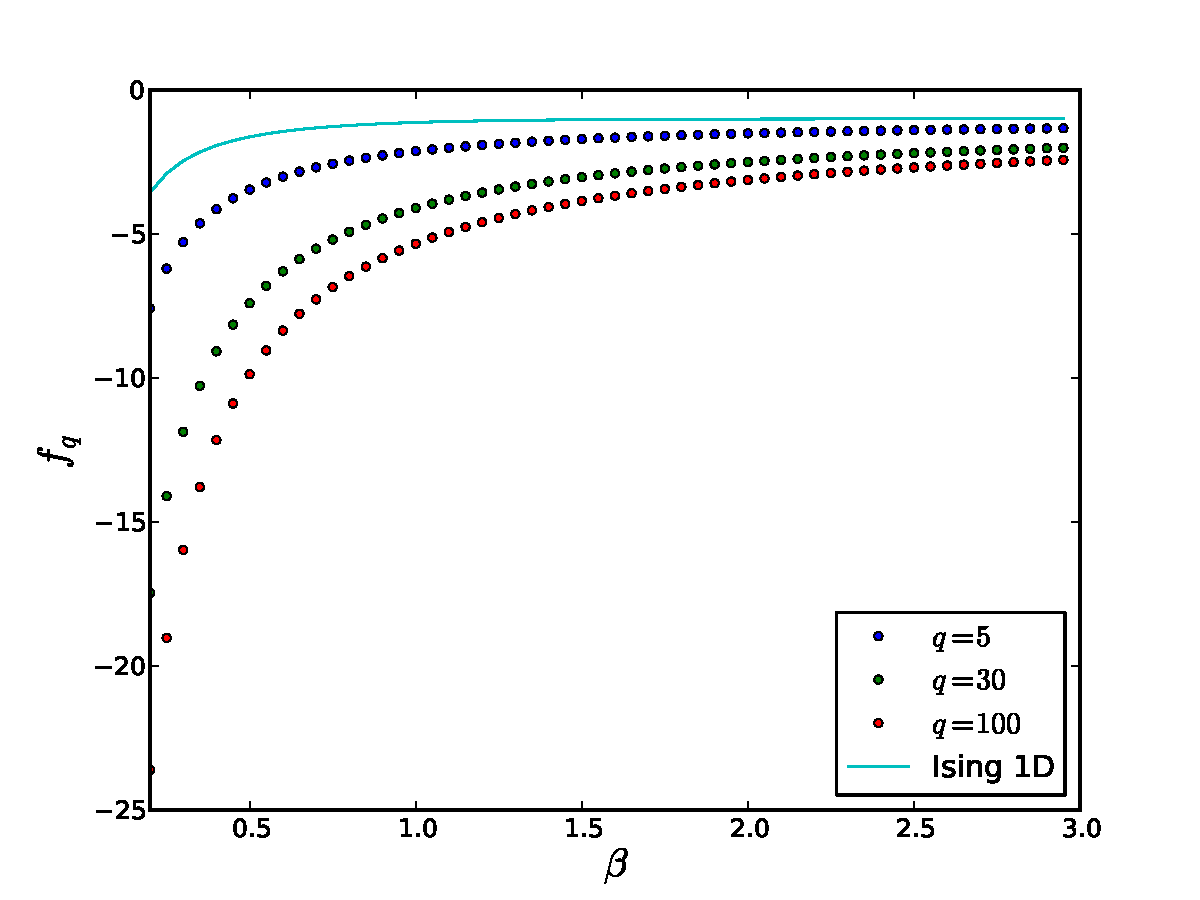
\includegraphics[scale=0.5]{Figures/f1d.pdf}
\caption{{\em Free energy of the 1d coprime model. The points are the numerical data obtained from exact diagonalization of \eqref{transfermatrix}. The solid curve represents the free energy of the 1d Ising model at zero external field.}}
\label{f1d}
\end{figure}
It is difficult to say whether or not it exists an analytic expression for $f_q(\beta)$. By the way it is worth noting that the largest eigenvalue of the transfer matrix \eqref{transfermatrix} scales as the number $q$ of integers per site and the limit $q \to \infty$ of the ratio $\lambda_\mathrm{max}/q$ is finite. Then the limit
\be \label{fun}
\lim_{q \to \infty } \[ - \beta f_q(\beta) - \log q \, \] = - \beta f(\beta)
\ee
defines an analytic function of $\beta$ independent of $q$. The value of this function when $\beta \to -\infty$ can actually be computed exactly, since
\be 
\lim_{\beta \to -\infty } T_{a,b}  = 1 - \phi(a,b) 
\ee
and the largest eigenvalue of the transfer matrix is given by the infinite product\footnote{Don Zagier, private communication}
\be 
\lim_{q \to \infty} \frac{ \lambda_\mathrm{max} }{ q } = \lim_{\beta \to -\infty} \exp \(-\beta f (\beta) \) = \prod_{p ~ \mathrm{prime} } \( \frac{ p-1 + \sqrt{(p-1)(p+3)} }{2 p}  \) \simeq 0.6784..
\ee
Let's now start switching on one at a time the couplings in the quantum Hamiltonian \eqref{quantumhamiltonian}, in such a way to make the model purely quantum. We will see that it is possible to reproduce the critical points of the universality classes of the $n$-state Potts model for $n=2,3,4$. This can be achieved thanks to the form of the coprime interaction, which allows one to select, among the exponential amount of ground states discussed above, only a finite number of them.\\ What follows is the outcome of a numerical diagonalization of the Hamiltonian \eqref{quantumhamiltonian} with $q=5$ and periodic boundary conditions\footnote{A potential critical behavior would not be affected by the boundary condition employed. Chosing the periodic one is simply a way to make the finite size scaling as fast as possible.}. Since the integer on each site assumes values between $2$ and $5$ the Hilbert space is $4^N$-dimensional for a chain of $N$ sites.

\vspace{3mm}
\noindent 
{\bf Ising model universality class}.
The critical point of the Ising model is well known to be described by the $\mathcal{M}_2$ minimal model, i.e. a conformal field theory whose central charge is $1/2$ \cite{bpz}. The critical behavior of this universality class does emerge e.g. at the transition point of the quantum Ising model in a transverse field, whose Hamiltonian reads
\be 
H \,=\,-\sum_{i=1}^N \left[ \sigma^z_i \sigma^z_{i+1} + h \sigma^x_i \right]  
\ee
Approaching the value $h=1$ this model undergoes a quantum phase transition which is made evident by the closure of the gap in the energy spectrum. Since this model can be solved exactly \cite{sachdev}, the central charge of this critical point can be calculated explicitly in many different ways. For instance it can be read from the scaling of the groud state energy with the number $N$ of sites of the chain \cite{bcn},\cite{aff}. However this method is of no use from a numerical point of view, as it implicitly requires the exact spectrum to be at hand. Since the spectrum of the quantum chain \eqref{quantumhamiltonian} is so far not known even for particular choices of the $B_\alpha$ operators, we need another way to get numerically the central charge. This can be achieved by looking at the finite size scaling of another numerically-computable quantity, namely the entanglement entropy of the ground state. Indeed it can be proven \cite{ccee} that for a critical one-dimensional spin chain of $N$ sites, with periodic boundary conditions, bipartite in two subchains $A$ and $B$ whose length is $n$ and $N-n$, the entanglement entropy of the ground state reads
\be \label{entent}
S_A (n) = -\tr \, \hat{\rho}_A \log \hat{\rho}_A = \frac{c}{3} \log \( \pi N \sin \frac{ \pi n}{N} \) + \mathrm{const}
\ee
where $\hat{\rho}_A$ is the ground state reduced density matrix of the subsystem $A$
\be
\hat{\rho}_A = \tr_B \( \ket{ GS } \bra{ GS } \)
\ee
and $c$ is the central charge. This formula can be used to fit numerical data for fixed number of sites $N$ or for fixed size of the subsystem $n=N/2$ varying $N$.\\
This said we have now to induce a transition via switching on some couplings $\lambda_\alpha$, place the Hamiltonian on the transition point and then measure the central charge as described above. The quantum critical point of the Ising model can be obtained using the following operators
\be \label{bope2}
B^1 = 
\begin{pmatrix}
1 & 0 & 0 & 0 \\
0 & 1 & 0 & 0 \\
0 & 0 & 0 & 0 \\
0 & 0 & 0 & 0 
\end{pmatrix}
\qquad
\qquad
B^2 = 
\begin{pmatrix}
0 & 1 & 0 & 0 \\
1 & 0 & 0 & 0 \\
0 & 0 & 0 & 0 \\
0 & 0 & 0 & 0 
\end{pmatrix}
\ee
so that the quantum Hamiltonian takes the form
\be \label{qh1}
H \,=\,-\sum_{i=1}^M \left[\Phi_{i,i+1}  +  \lambda_1 B^1_i   + \lambda_2 B^2_i \right] 
\ee
The first one-site operator is necessary to favour the two states $\ket{2}$, $\ket{3}$, in order to pick the two unique ground states of the whole chain
\be 
\ket{2\,2\,2\,2\,\dots 2}
\qquad \qquad
\ket{3\,3\,3\,3\,\dots 3}
\ee
Note that, although the ground state level is the one above irrespective of the value of $\lambda_1$, the latter affects the first excited level. In fact the energy of the zero-level is $E_{GS} = - (1+\lambda_1)N$, while the best candidates for the first-level are the $N$-degenerate state
\be \label{n-deg}
\ket{ 2 \, 2 \, \dots 2 \, 4 \, 2 \, \dots 2 }
\ee
whose energy is $E_1 = - N - (N-1) \lambda_1$, and the $N(N-1)/2$-degenerate two-domain walls level
\be \label{2p-deg}
\ket{ 2 \, 2 \, \dots 2 \, 3 \, \dots 3 \, 2 }
\ee
whose energy is $E_2 = -(N-2) - N \lambda_1$. Then if $\lambda_1 < 2$ one has $E_1 < E_2$ and the first excited states are \eqref{n-deg}, while if $\lambda_1 > 2$ the states in \eqref{2p-deg} become the first level. 
%%%This shows that the low energy spectrum changes structure when $\lambda_1$ is varyied. Nonetheless in both cases the switching of the second operator in \eqref{bope2} leads to a quantum phase transition for the finite value of $\lambda_2 = 0.5$. This can be seen from the analysis of the ground state degeneracy, which is preserved (up to terms exponentially small in $N$) up to the value $\lambda_2 = 0.5$, where it is definetly broken to leave only one non-degenerate ground state. Moreover one can study the energy gap of the quantum Hamiltonian \eqref{qh1}, i.e. the difference between the eigenvalue of the first excited state and of the ground state $\Delta E = E_{1st} - E_{GS}$, as a function of $\lambda_2$ for fixed $\lambda_1$. The result is shown in Figure \ref{gap2}.%%%


\begin{figure}[H]
\center
\makebox[0pt][c]{
\hspace{-10mm}
\begin{minipage}{0.52\textwidth}
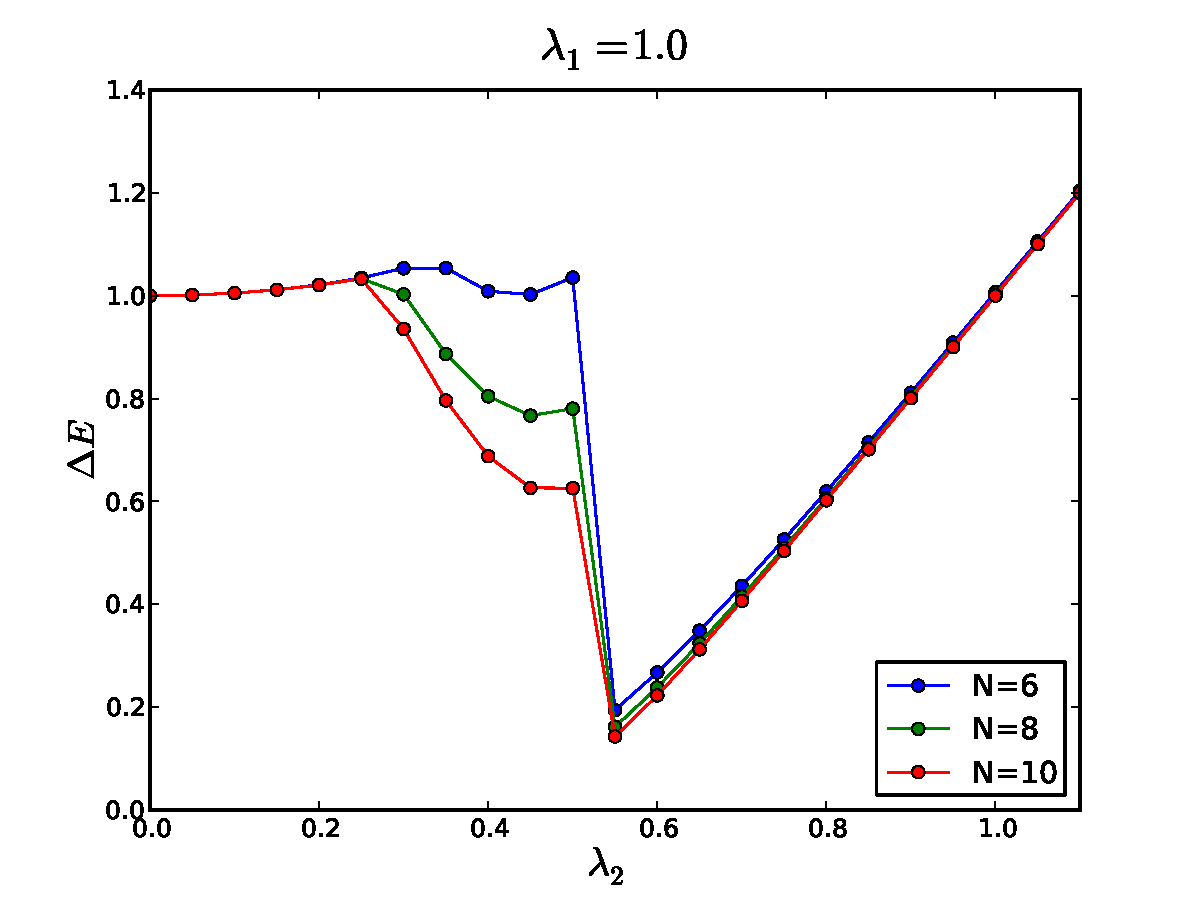
\includegraphics[scale=0.45]{Figures/gap2.pdf}
\end{minipage}
\begin{minipage}{0.53\textwidth}
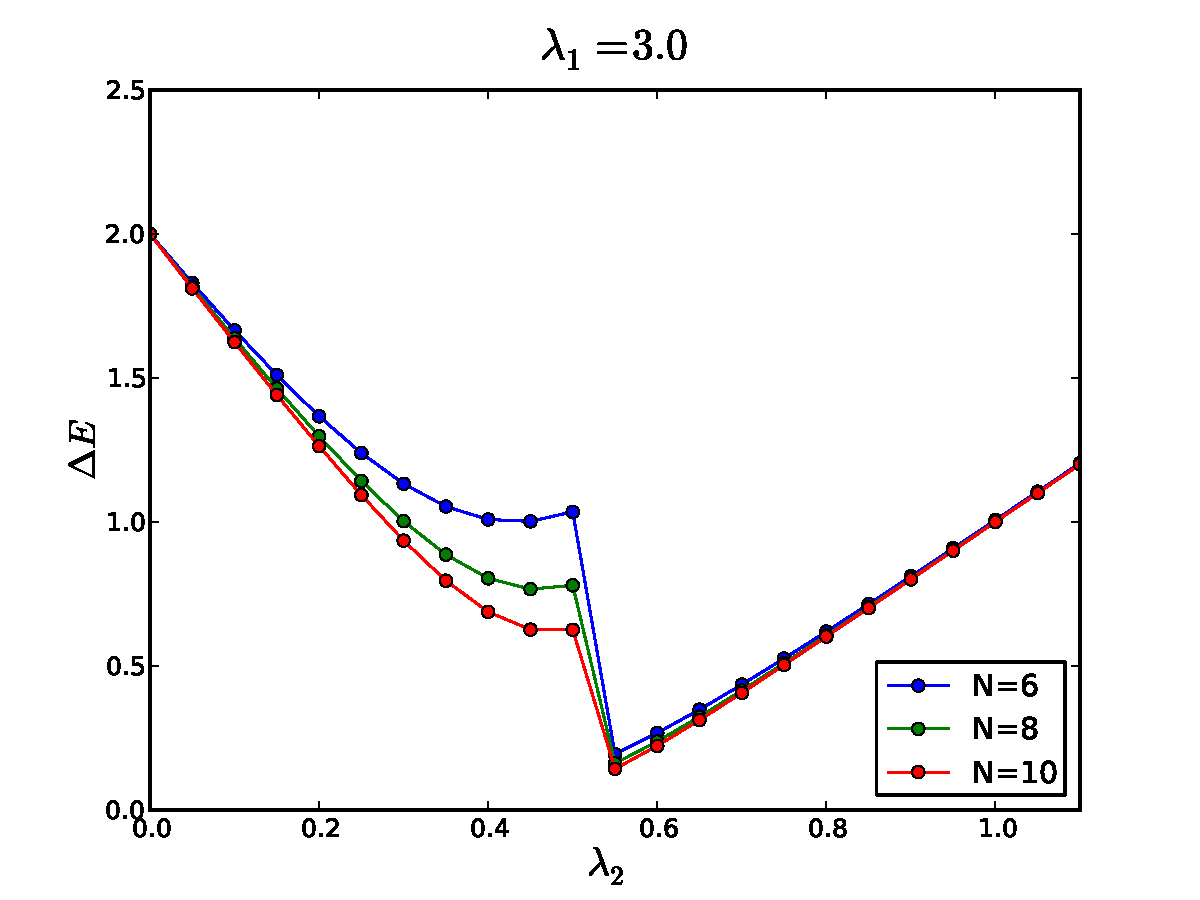
\includegraphics[scale=0.45]{Figures/gap22.pdf}
\end{minipage}}
\caption{{\em Gap of the quantum Hamiltonian with $B_1$ and $B_2$, for fixed $\lambda_1=1.0,3.0$ and varying $\lambda_2$. The finite size scaling shows the closure of the gap when $\lambda_2 \simeq 1/2$, independently of the value of $\lambda_1$. Then the QPT occurs because of the structure of the ground state level. }}
\label{gap2}
\end{figure}
\noindent
Once the transition point has been located we can identify the universality class of this QPT using the technique described above. As depicted in Figure \ref{ee2} and Figure \ref{ee22} the transition point is critical, since the entanglement entropy diverges logarithmically with the $N$, and the central charge is $c = 1/2$, which is the one of the Ising universality class.  

\begin{figure}[H]
\center
\makebox[0pt][c]{
\hspace{-15mm}
\begin{minipage}{0.33\textwidth}
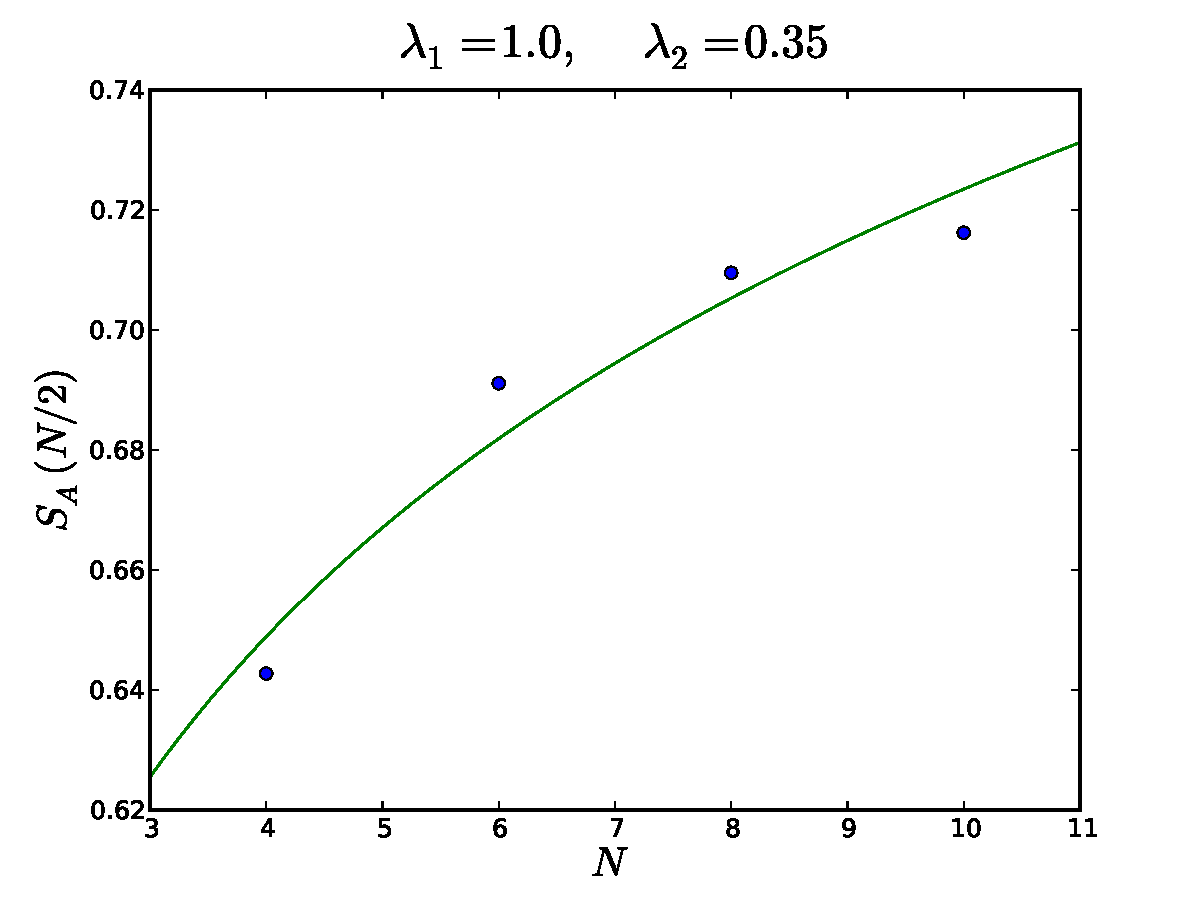
\includegraphics[scale=0.32]{Figures/ee21_35.pdf}
\end{minipage}
\hspace{4mm}
\begin{minipage}{0.33\textwidth}
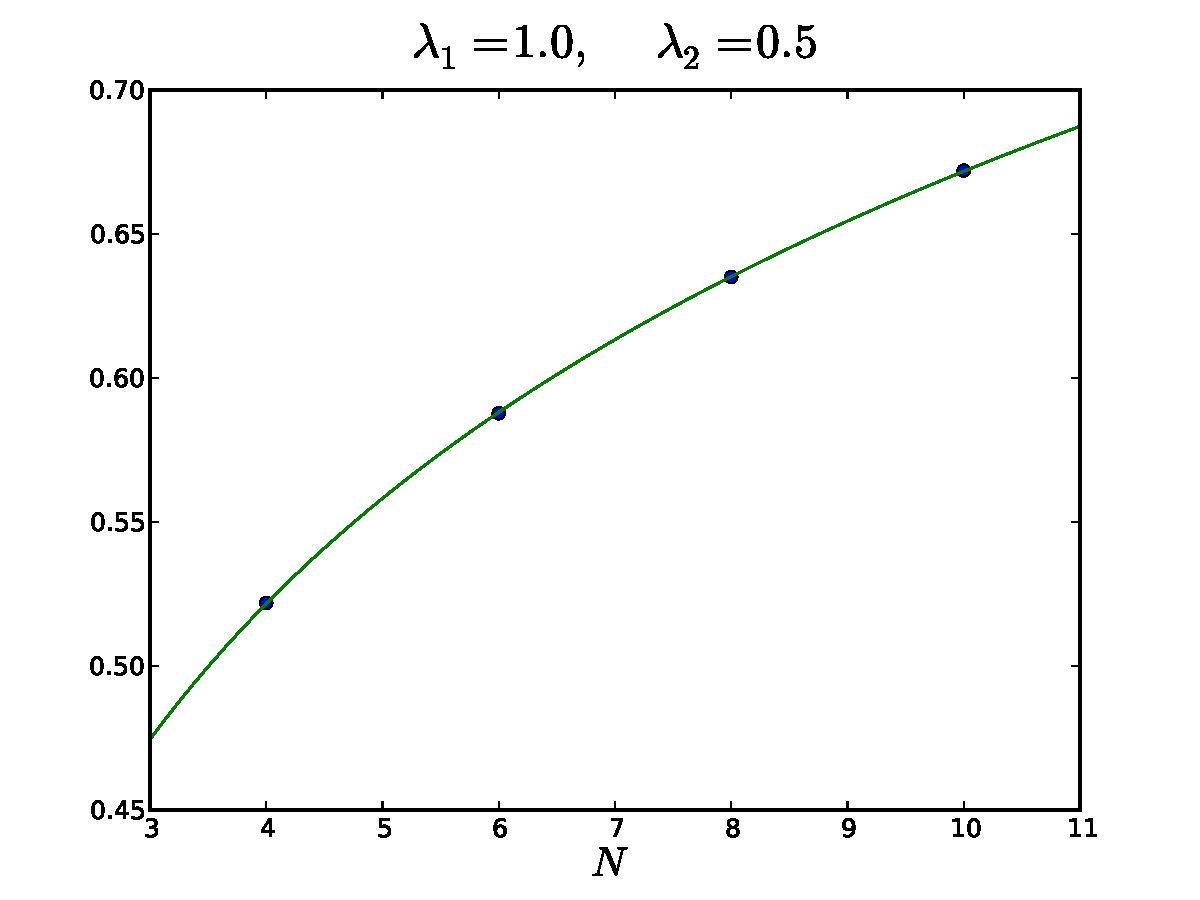
\includegraphics[scale=0.32]{Figures/ee21_50.pdf}
\end{minipage}
\hspace{4mm}
\begin{minipage}{0.33\textwidth}
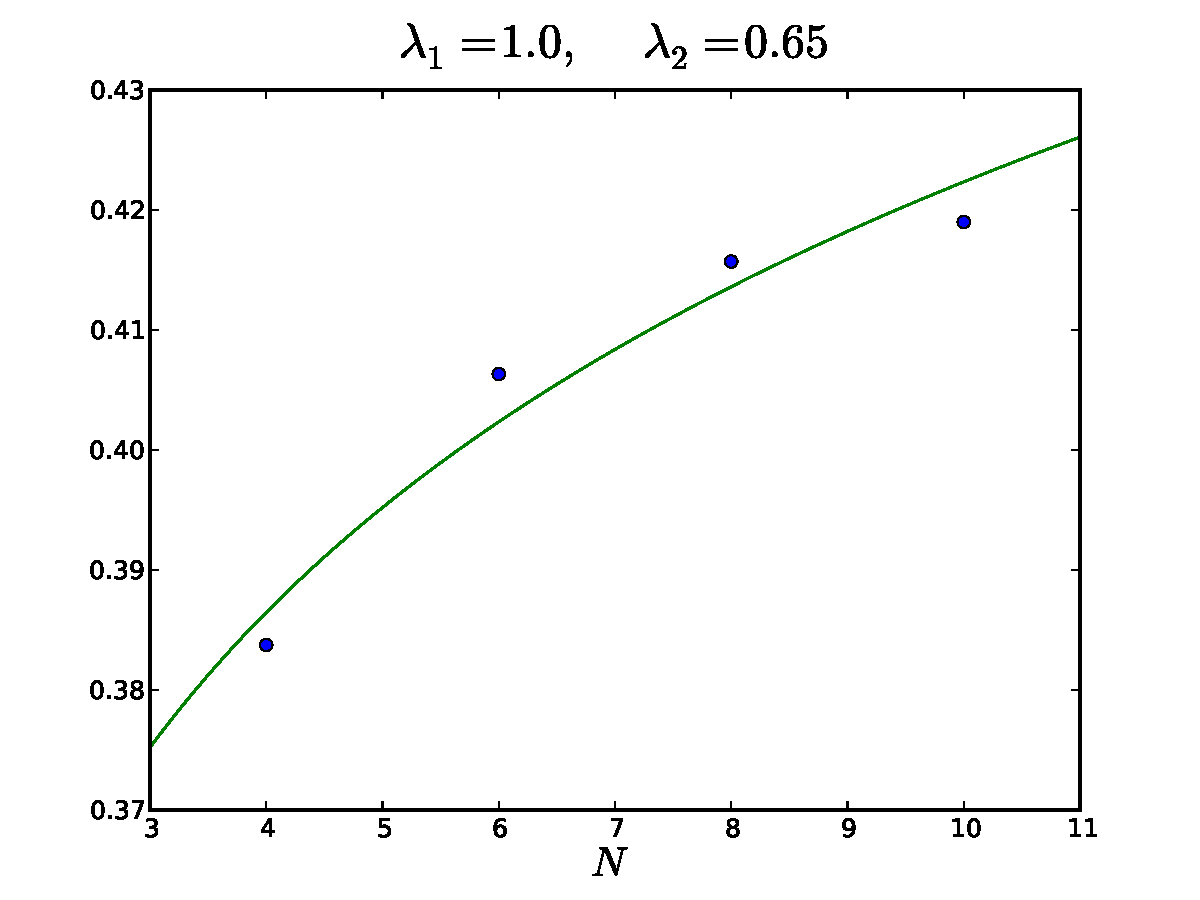
\includegraphics[scale=0.32]{Figures/ee21_65.pdf}
\end{minipage}}\\
\makebox[0pt][c]{
\hspace{-15mm}
\begin{minipage}{0.33\textwidth}
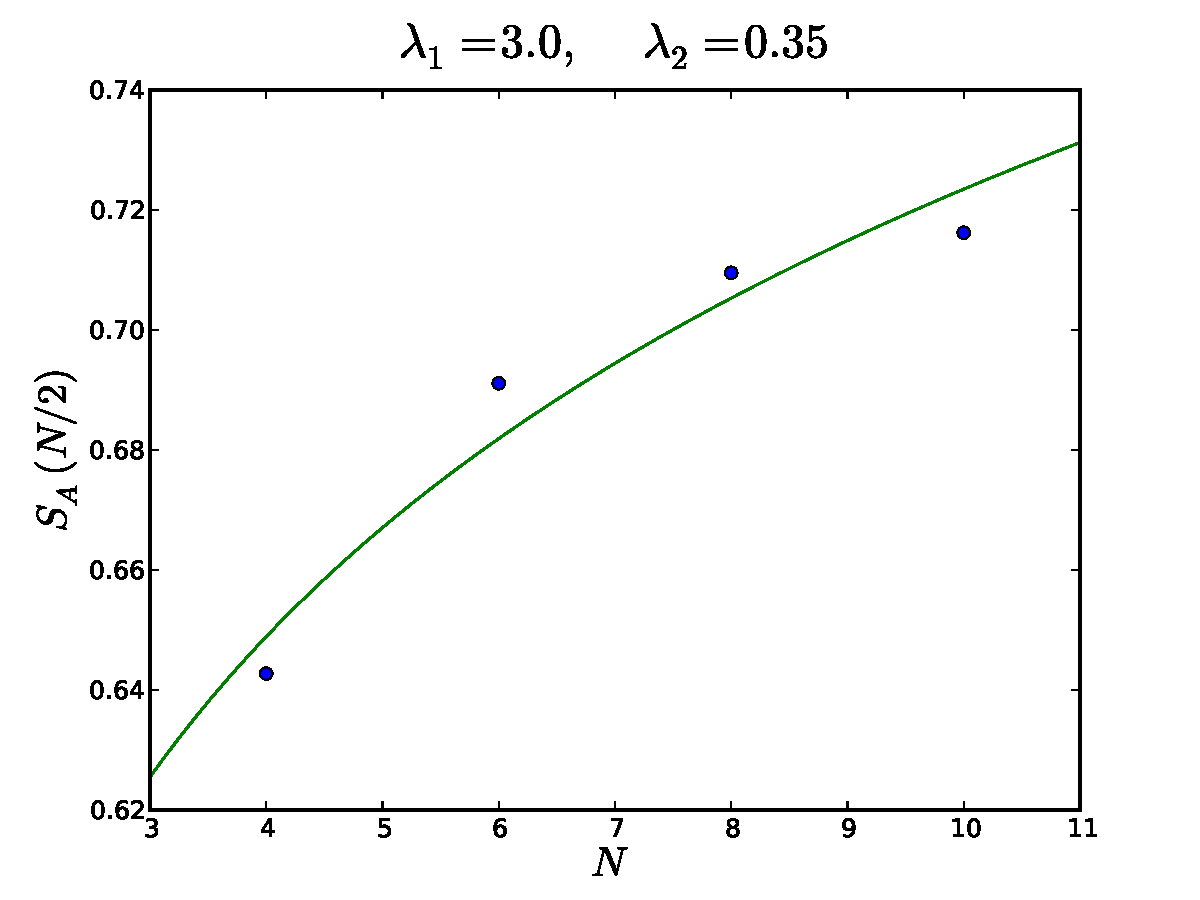
\includegraphics[scale=0.32]{Figures/ee23_35.pdf}
\end{minipage}
\hspace{4mm}
\begin{minipage}{0.33\textwidth}
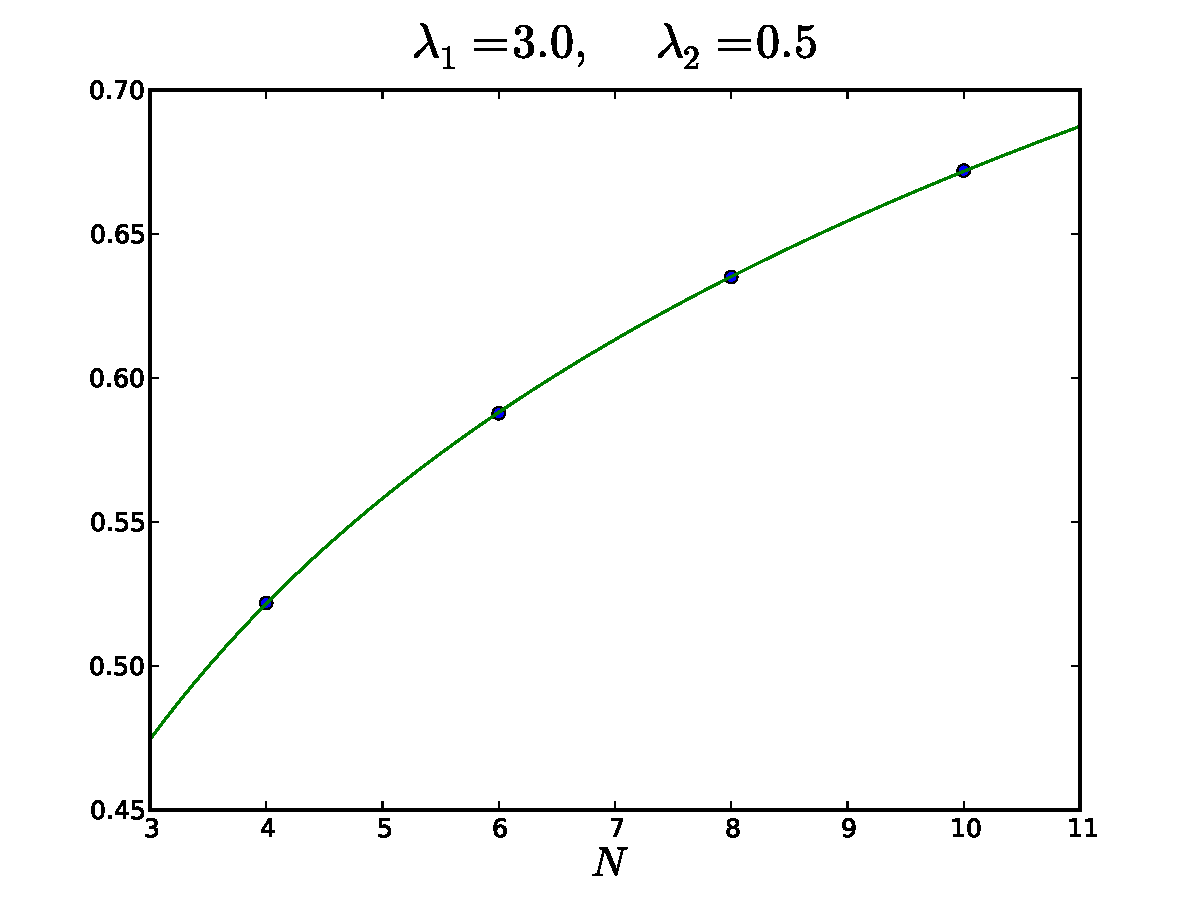
\includegraphics[scale=0.32]{Figures/ee23_50.pdf}
\end{minipage}
\hspace{4mm}
\begin{minipage}{0.33\textwidth}
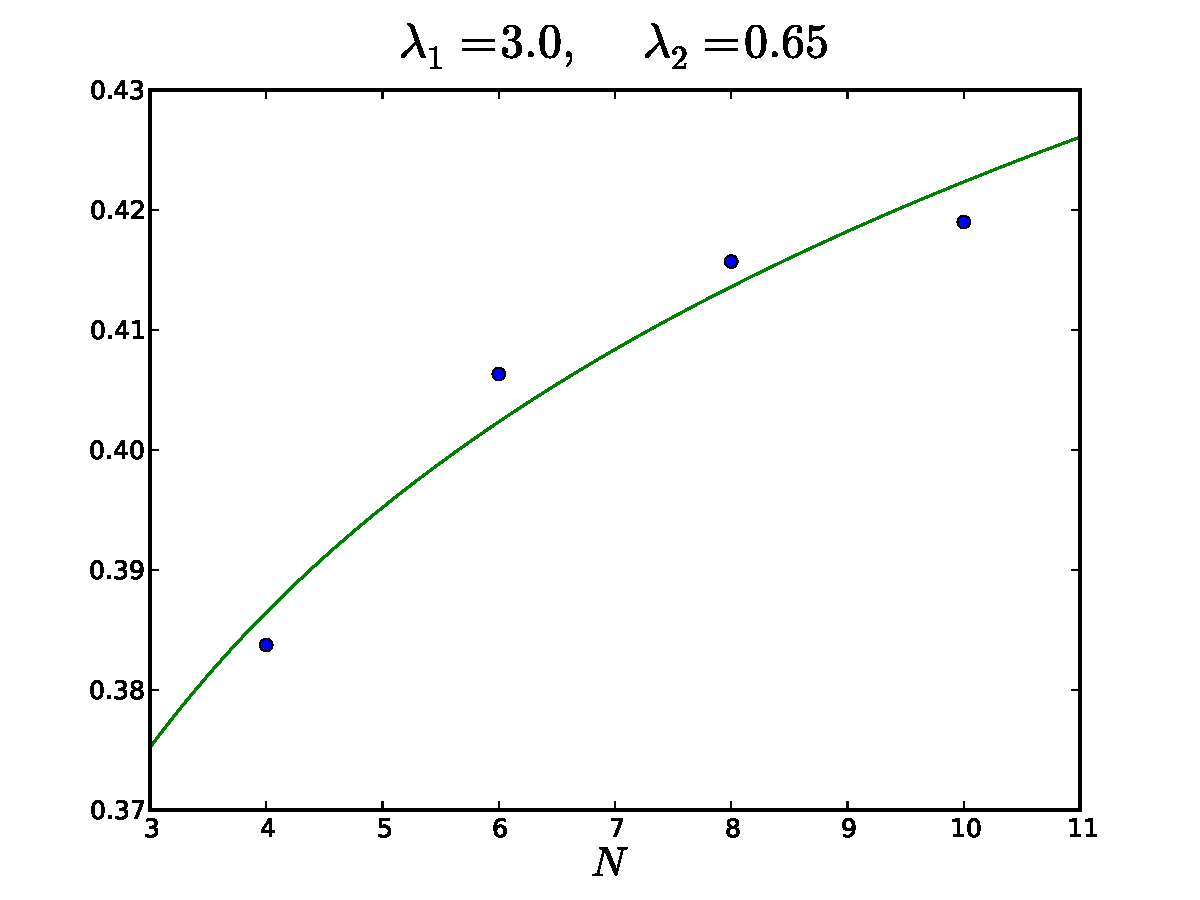
\includegraphics[scale=0.32]{Figures/ee23_65.pdf}
\end{minipage}}
\caption{{\em Finite size scaling of the entanglement entropy near the transition point $\lambda_2 = 1/2$. The scaling of the data in the plot in the middle fit \eqref{entent} very well with $c=0.4915..$, when either $\lambda_1=1.0$ or $\lambda_1=3.0$. As soon as $\lambda_2$ detaches from the critical value the entanglement entropy saturates very rapidly to a value proportional to the logarithm of the correlation length.}}
\label{ee2}
\end{figure}
\begin{figure}[H]
\center
\makebox[0pt][c]{
\hspace{-10mm}
\begin{minipage}{0.52\textwidth}
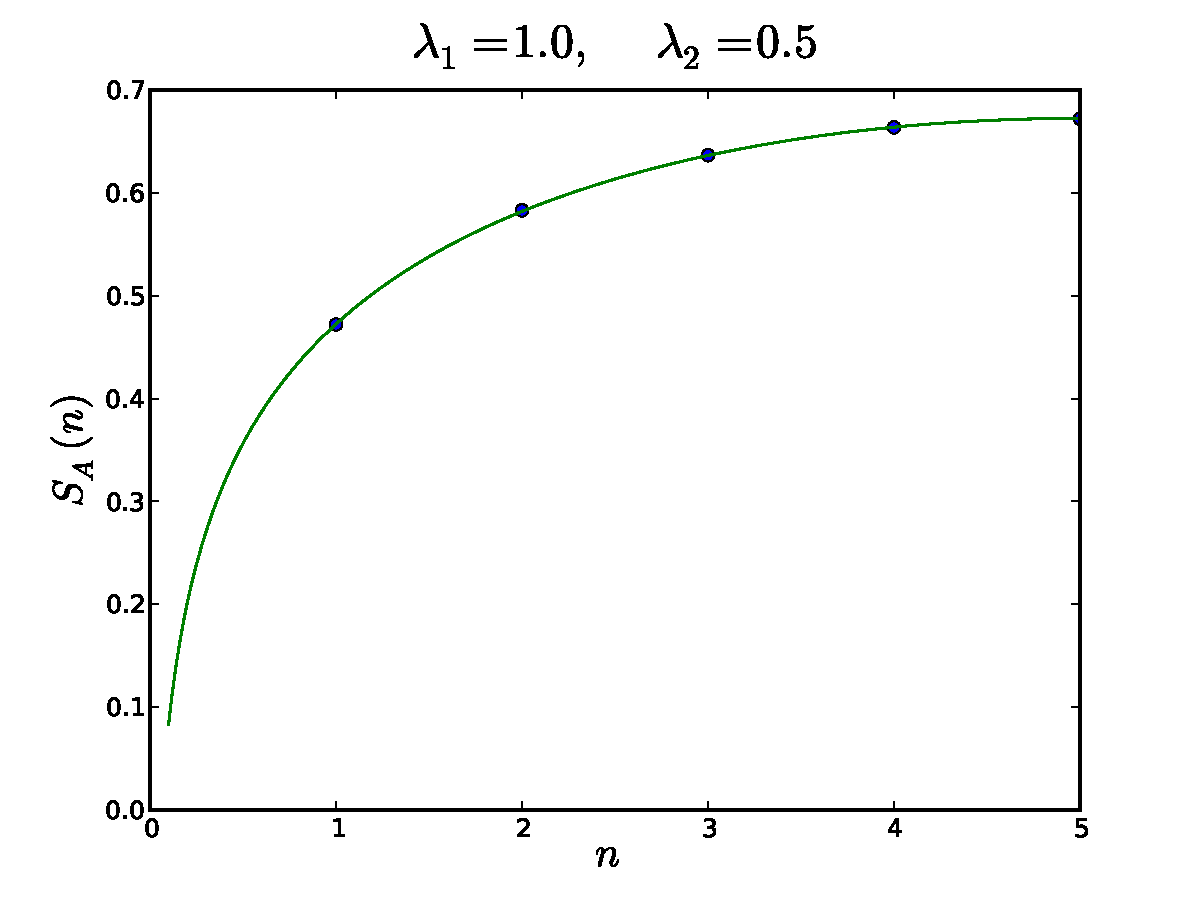
\includegraphics[scale=0.45]{Figures/ee221_50.pdf}
\end{minipage}
\begin{minipage}{0.53\textwidth}
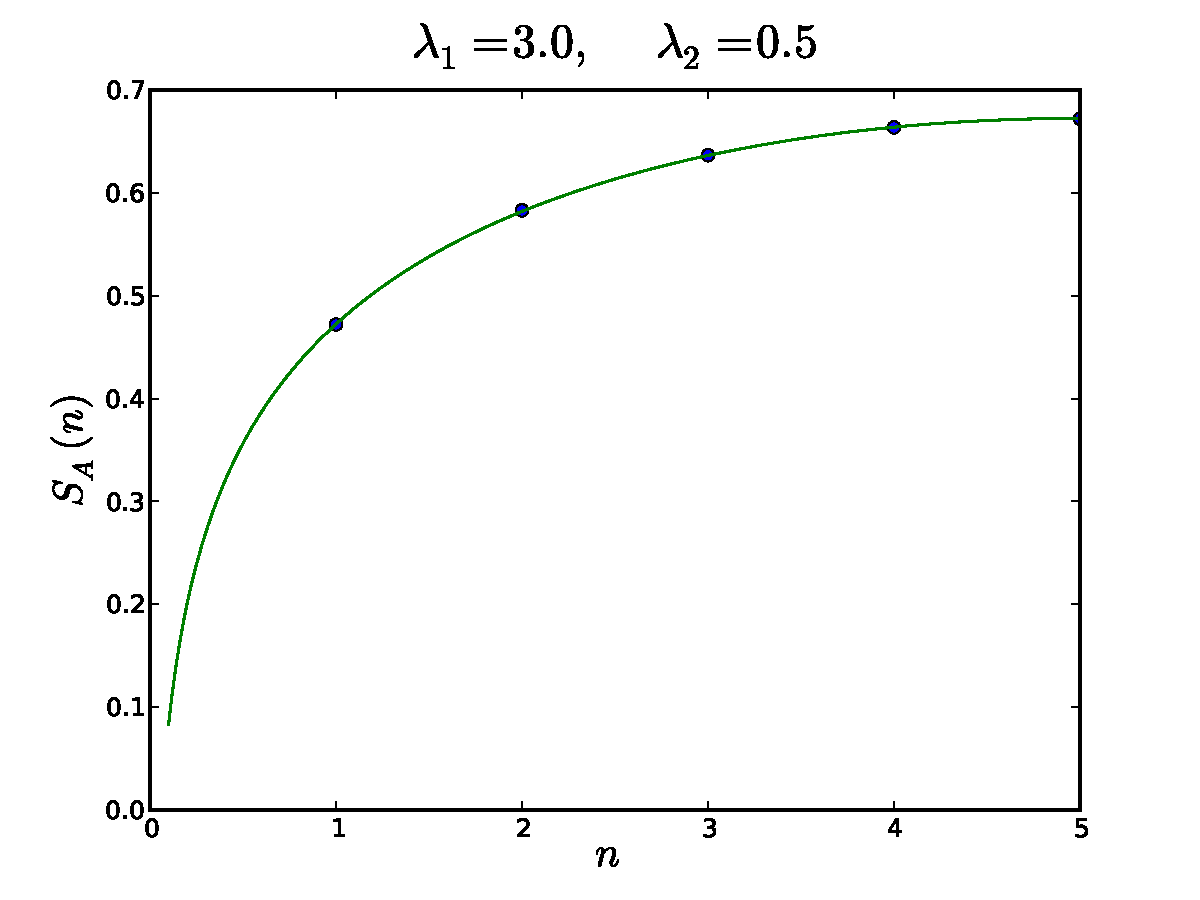
\includegraphics[scale=0.45]{Figures/ee223_50.pdf}
\end{minipage}}
\caption{{\em Entanglement entropy for a chain of $N=10$ sites, varying the size $n$ of the subsystem $A$ at the transition point $\lambda_2 = 1/2$. The fit with \eqref{entent} produces the value of the central charge $c=0.510..$ both when $\lambda_1=1.0$ and when $\lambda_2=3.0$. }}
\label{ee22}
\end{figure}

[Note about symmetry? (selecting 2 and 3 the Hamiltonian is not invariant under the permutation of the state $\ket{2}$ and $\ket{3}$ since the interaction is not. Nevertheless the transition point seems to be the conformal one associated to the permutation symmetry of $2$ elements)] 

\vspace{3mm}
\noindent 
{\bf 3-states Potts model universality class}. It is possible to play in the same way with the operators $B_\alpha$ in \eqref{quantumhamiltonian} to realize other critical points belonging to various universality classes. For example the critical behavior of the $3$-states Potts model, which is described by a CFT whose central charge is $c=4/5$ \cite{dots}, can be reproduced in the quantum coprime chain in a similar way as before. First we have to pull down $3$ ground states from the exponentially degenerate zero level of the coprime interaction. Once we have the discrete number of ground states we can mix the one-site states with increasing strength $\lambda_2$ in such a way to produce a QPT at a finite non-zero value of this coupling. The operators which do the job for $n=3$ are the following
\be 
B^1 = 
\begin{pmatrix}
1 & 0 & 0 & 0 \\
0 & 1 & 0 & 0 \\
0 & 0 & 0 & 0 \\
0 & 0 & 0 & 1 
\end{pmatrix}
\qquad
\qquad
B^2 = 
\begin{pmatrix}
0 & 1 & 0 & 1 \\
1 & 0 & 0 & 1 \\
0 & 0 & 0 & 0 \\
1 & 1 & 0 & 0 
\end{pmatrix}
\ee
The ground state level this time is generated by the states
\be \label{inertgs}
\ket{2\,2\,2\,2\,\dots 2}
\qquad \qquad
\ket{3\,3\,3\,3\,\dots 3}
\qquad \qquad
\ket{5\,5\,5\,5\, \dots 5}
\ee
As before the first excited level changes when $\lambda_1$ overcomes the value of $2.0$, but the critical behavior is not affected. We can infer about the location of the transition point and its conformal invariance from the analysis of the energy gap of the Hamiltonian varying $\lambda_2$ and form the scaling of the entanglement entropy respectively. The critical point is located at $\lambda_2 = 1/3$ and the measure of the central charge is compatible with the value $c=4/5$, which is the one the $3$-states Potts model universality class. The numerical results are reported in Figure \ref{gap3} and Figure \ref{ee3}.


\begin{figure}[H]
\center
\makebox[0pt][c]{
\hspace{-10mm}
\begin{minipage}{0.52\textwidth}
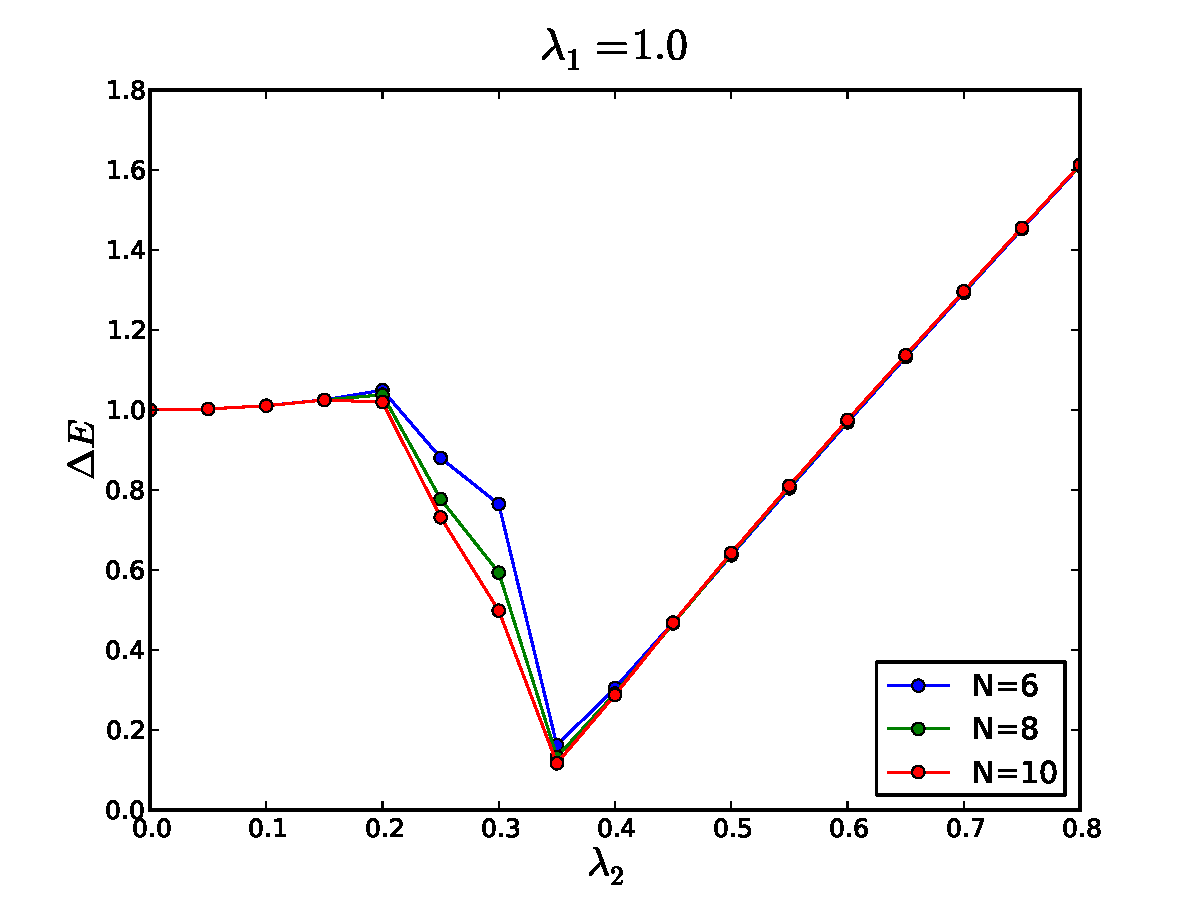
\includegraphics[scale=0.45]{Figures/gap3.pdf}
\end{minipage}
\begin{minipage}{0.53\textwidth}
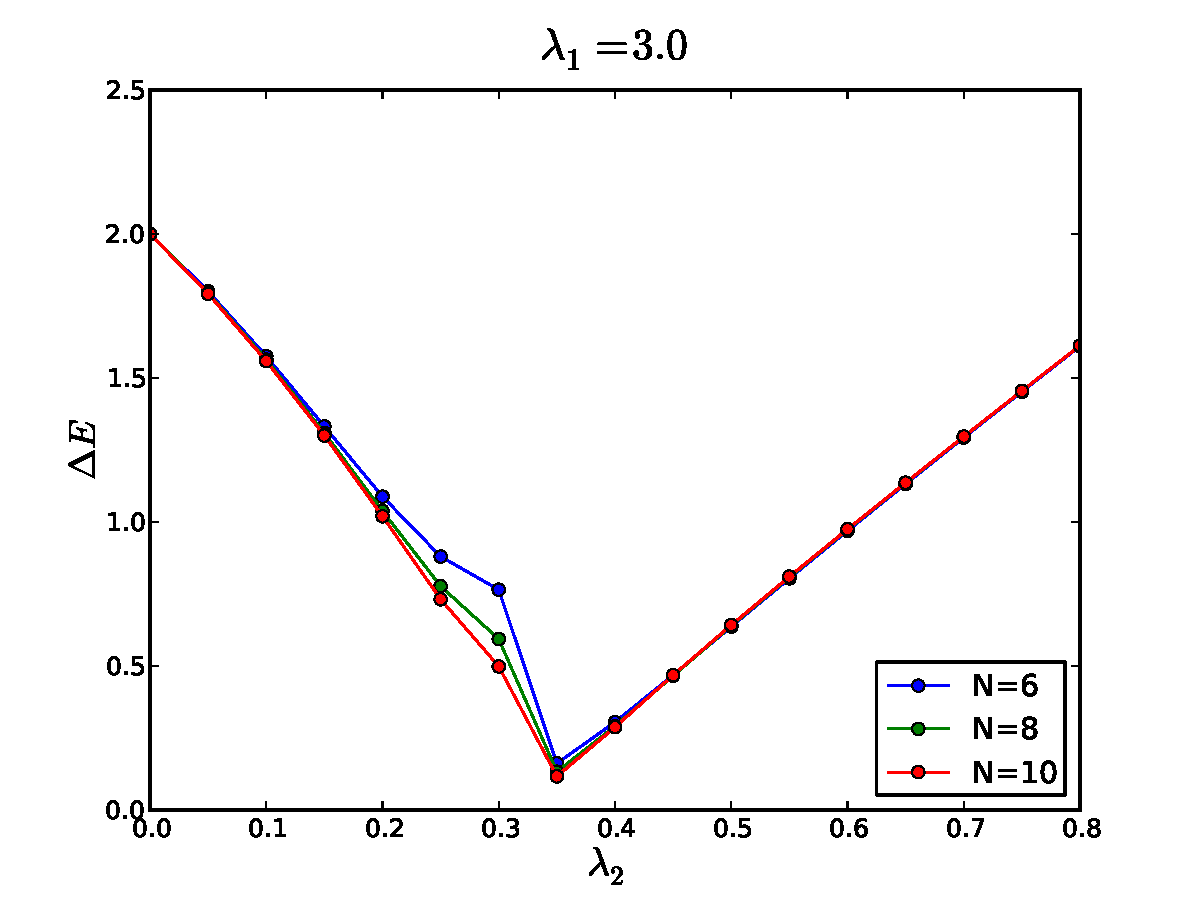
\includegraphics[scale=0.45]{Figures/gap32.pdf}
\end{minipage}}
\caption{{\em Gap of the quantum Hamiltonian with $B_1$ and $B_2$, for fixed $\lambda_1=1.0,3.0$ and varying $\lambda_2$. The finite size scaling shows the closure of the gap when $\lambda_2 \simeq 1/3$, independently of the value of $\lambda_1$. }}
\label{gap3}
\end{figure}

\begin{figure}[H]
\center
\makebox[0pt][c]{
\hspace{-10mm}
\begin{minipage}{0.52\textwidth}
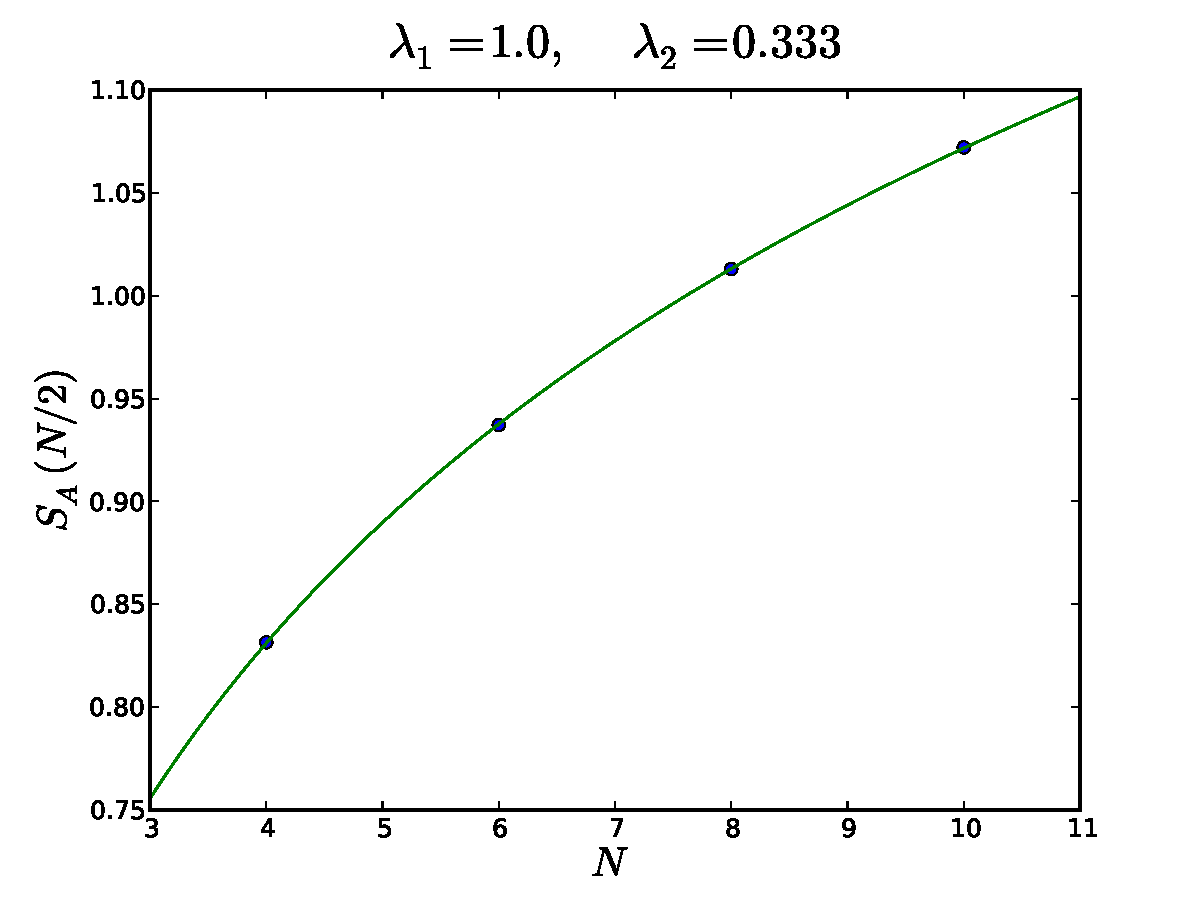
\includegraphics[scale=0.45]{Figures/ee31_33.pdf}
\end{minipage}
\begin{minipage}{0.53\textwidth}
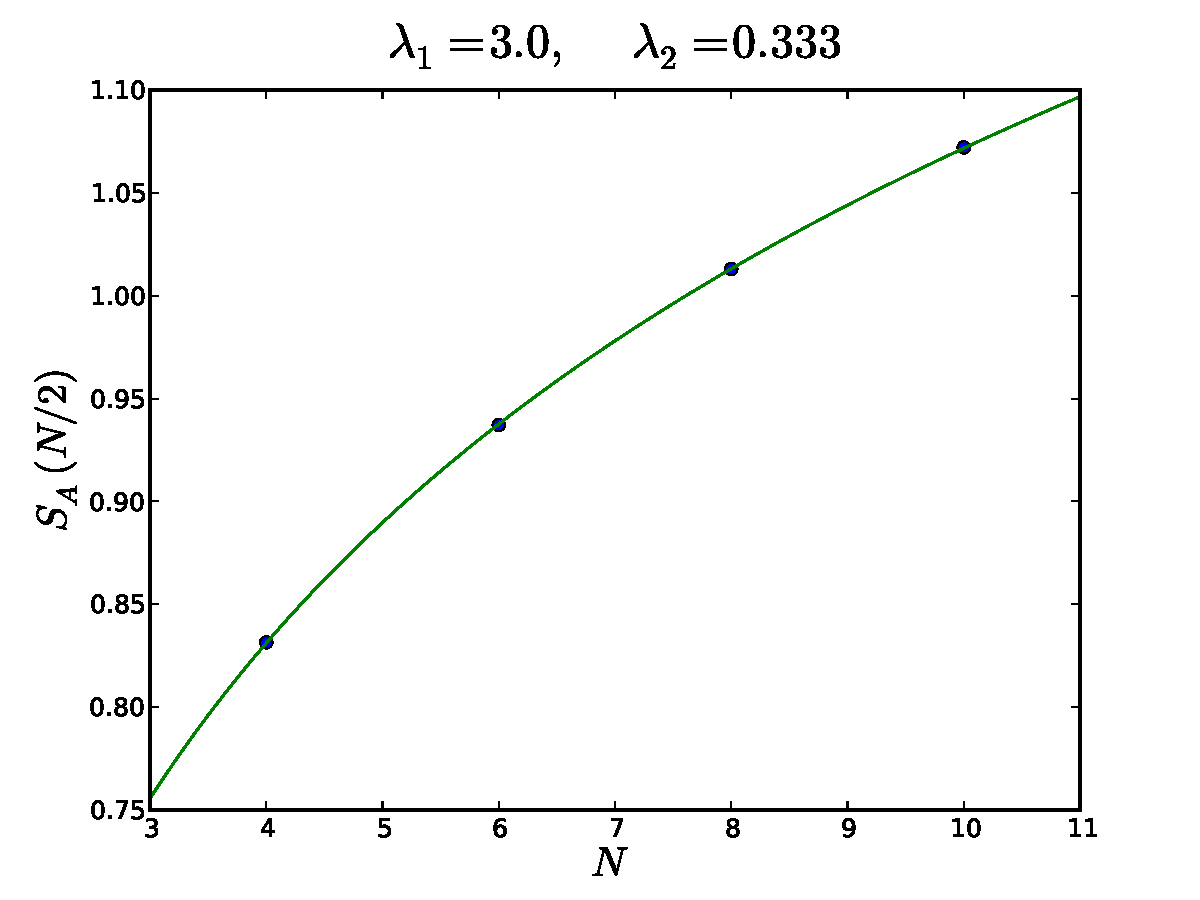
\includegraphics[scale=0.45]{Figures/ee33_33.pdf}
\end{minipage}}
\caption{{\em Finite size scaling of the entanglement entropy at the transition point $\lambda_2 = 1/3$. The fit with \eqref{entent} gives a central charge $c=0.7876,,$ independently of $\lambda_1$. }}
\label{ee3}
\end{figure}

\begin{figure}[H]
\center
\makebox[0pt][c]{
\hspace{-10mm}
\begin{minipage}{0.52\textwidth}
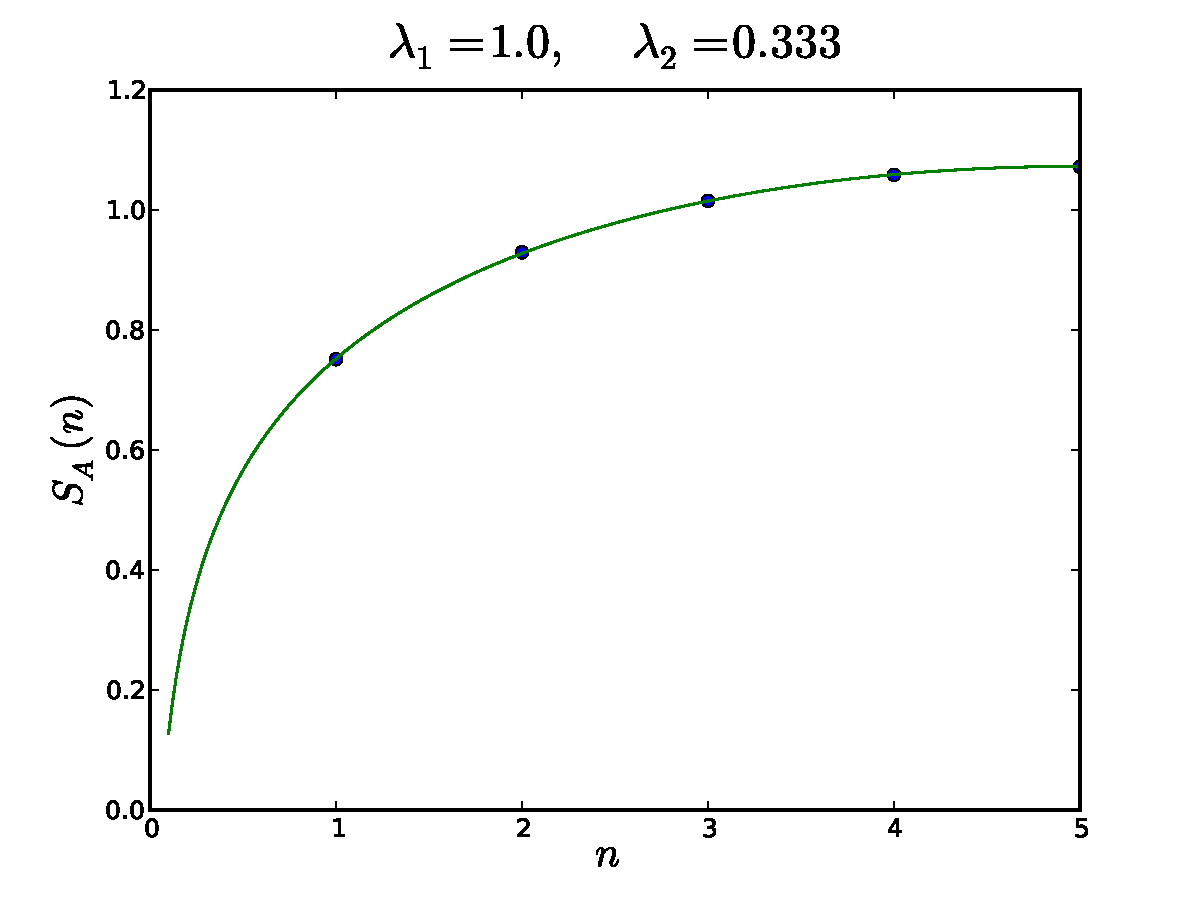
\includegraphics[scale=0.45]{Figures/ee321_33.pdf}
\end{minipage}
\begin{minipage}{0.53\textwidth}
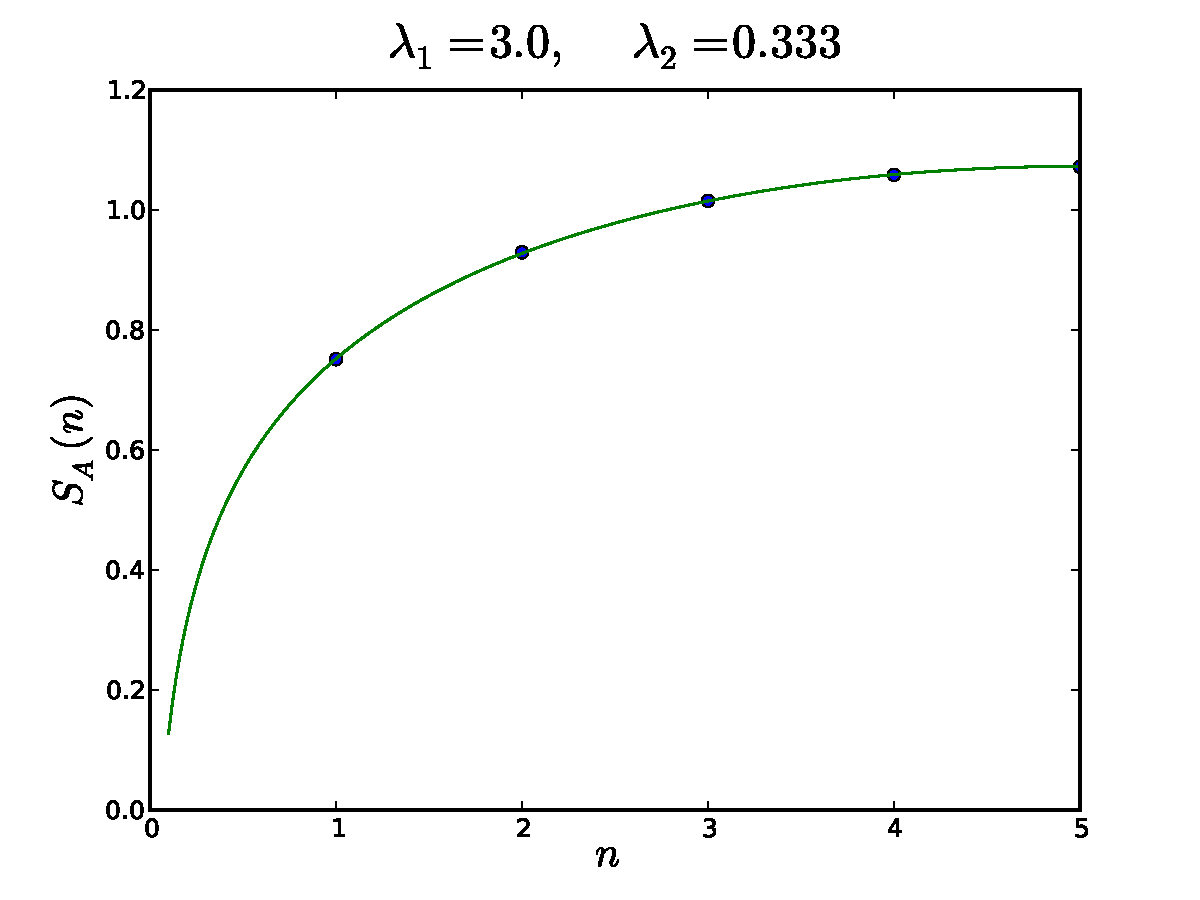
\includegraphics[scale=0.45]{Figures/ee323_33.pdf}
\end{minipage}}
\caption{{\em Entanglement entropy for a chain of $N=10$ sites, $\lambda_1=1.0,3.0$, varying the size $n$ of the subsystem $A$ at the transition point $\lambda_2 = 1/2$. The fit with \eqref{entent} produces the value of the central charge $c=0.8194..$ both when $\lambda_1=1.0$ and when $\lambda_2=3.0$. }}
\label{ee32}
\end{figure}


\vspace{3mm}
\noindent 
{\bf No QPT with an exponential number of ground states}. We can play the same way with the single-site states $\ket{2}$ and $\ket{4}$. Lowering their energy we simply remove the two inert ground states $\ket{3\,3\,3\, \dots 3 }$ and $\ket{5\,5\,5\, \dots 5 }$ from the exponentially degenerate zero level of the coprime interaction. We can then mix the states $\ket{2}$ and $\ket{4}$, with an operator similar to the $B^2$s above, and look for quantum phase transitions for finite values of $\lambda_2$. This is realized turning on the following operators
\be 
B^1 = 
\begin{pmatrix}
1 & 0 & 0 & 0 \\
0 & 0 & 0 & 0 \\
0 & 0 & 1 & 0 \\
0 & 0 & 0 & 0 
\end{pmatrix}
\qquad
\qquad
B^2 = 
\begin{pmatrix}
0 & 0 & 1 & 0 \\
0 & 0 & 0 & 0 \\
1 & 0 & 0 & 0 \\
0 & 0 & 0 & 0 
\end{pmatrix}
\ee
Contrary to what happened before, this time the ordered phase characterized by the ground state degeneracy does not survive to the mixing term, even for small values of $\lambda_2$, as depicted in Figure \ref{gap4}.
\begin{figure}[H]
\center
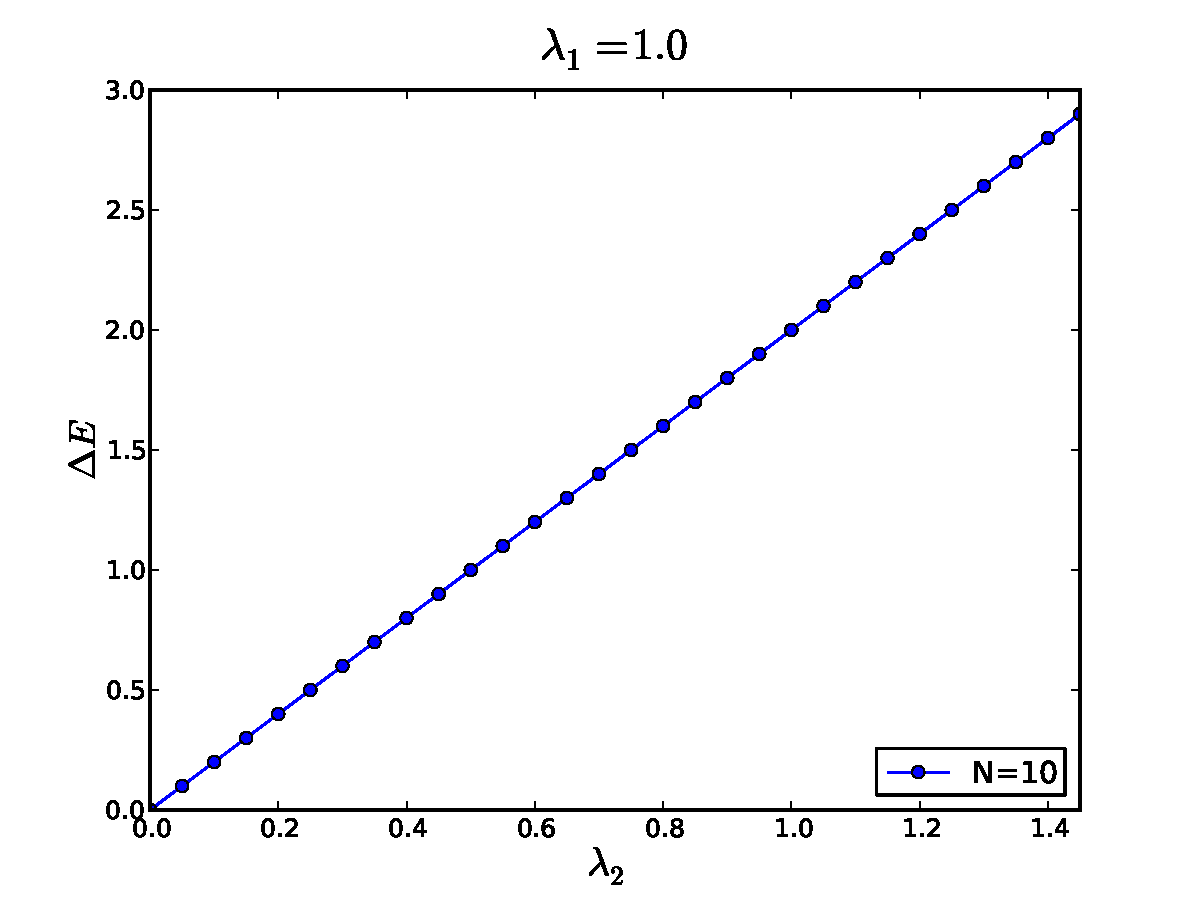
\includegraphics[scale=0.5]{Figures/gap4.pdf}
\caption{{\em Gap of the quantum Hamiltonian with $B_1$ and $B_2$, for fixed $\lambda_1=1.0$ and varying $\lambda_2$, on a chain of $N=10$ sites. The gap opens as soon as $\lambda_2$ is nonzero. Moreover $\Delta E$ depends linearly on $\lambda_2$ as $\Delta E = 2 \lambda_2$, indicating that perturbation theory is exact at first order. }}
\label{gap4}
\end{figure}
\noindent
This fact can be explained already at first order in perturbation theory. In fact treating the term with $B^2$ as a perturbation
\be \label{pert}
H_p = -\lambda_2 \sum_{i=1}^N B^2_i
\ee
and writing down its matrix elements in the $2^N$-degenerate ground state subspace composed of all the factorized states which are product of $\ket{2}$ and $\ket{4}$, it is easy to realize that the matrix one has to diagonalize in order to find the splitting of this energy level is (apart from the overall factor $-\lambda_2$) the one associated to a regular graph of degree $N$. Indeed acting with \eqref{pert} on a state made up of $2$s and $4$s one obtains $N$ different states of the same subspace. Then each row of the perturbation in this subspace will contain $N$ nonzero entries all equal to $-\lambda_2$ and the remaining $2^N - N$ entries equal to zero. Since this regular graph is also connected it follows, via Perron-Frobenius theorem, that the lowest eigenvalue is unique and equal to $-N \lambda_2$. This implies that the first order correction completly removes the ground state degeneracy, explaing the sudden opening of the gap as soon as $\lambda_2 \ne 0$. It is worth noting that this is contrast to what happens in the case when the ground state subspace has only a finite degeneracy in the $N \to \infty$ limit, as in the case of the $n$-state Potts model. There the transverse field has all zero entries in the subspace relative to the lowest eigenvalue of the unperturbed Hamiltonian, thus there is no splitting of zero level.\\
Although the graph theory-argument is pretty elegant and concise, it gives no information on the gap of $H_p$ in the thermodynamic limit. Indeed the spectral gap of a regular graph might even close when the number of vertices goes to infinity. However it is easy to write down the whole spectrum of $H_p$ in the degenerate subspace for every $N$. First observe that $H_p$ restricted to the ground state subspace is simply given by
\be 
\left. H_p \right|_{GS} = -\lambda_2 \sum_{i=1}^N \sigma^x_i
\ee
where $\sigma_x$ is the usual Pauli matrix whose eigenvectors will be denoted
\be 
\ket{ + } = \frac{1}{\sqrt{2}} \begin{pmatrix}
1 \\ 1
\end{pmatrix}
\qquad \qquad \qquad 
\ket{ - } = \frac{1}{\sqrt{2}} \begin{pmatrix}
1 \\ -1
\end{pmatrix}
\ee
Then one can construct the spectrum of $H_p$ starting form the product state $\ket{ + \, + \, + \, \dots + }$, which is the unique eigenstate associated to the lowest eigenvalue $-\lambda_2 N$, and flipping one spin at a time. In this way it is easy to realize that all the eigenvalues are organized as
\begin{align*}
 & E_{ + \, + \, + \, \dots + } = -\lambda_2 N  & \qquad    \qquad &  1-\mathrm{degenerate} & \\[2.5mm]
 & E_{ + \, + \, \dots  + \, - \, + \dots + } = -\lambda_2 (N-2)  & \qquad  \qquad & N-\mathrm{degenerate} & \\[1mm]
 & E_{ + \, + \, \dots  + \, - \, - \, + \dots + } = -\lambda_2 (N-4)  & \qquad  \qquad &  \binom{N}{2}-\mathrm{degenerate} & \\
 &  \qquad \qquad \vdots &  &  \qquad  \qquad  \vdots  & \\
 & E_{ + \, + \, \dots  + \, -  \, \dots \, - \, + \dots + } = -\lambda_2 (N-2 p)&  \qquad   \qquad & \binom{N}{p}-\mathrm{degenerate} & \\
 &  \qquad \qquad \vdots &  &  \qquad  \qquad  \vdots  & \\[1.5mm]
 & E_{ - \, - \, - \, \dots - } = \lambda_2 N  & \qquad    \qquad &  1-\mathrm{degenerate} & 
\end{align*}
Thus the gap is given by $\Delta E = 2 \lambda_2$ for any $N$. Moreover from the data in Figure \ref{gap4} it is clear that this does hold to all order.





\section{Classical 2d model and Hamiltonian limit}
From the discussion in the previous section it is clear that for particular choices of the operators $B^\alpha$ the quantum Hamiltonian is gapped for any nonzero value of the corresponding coupling $\lambda_\alpha$. Another possible choice producing a model with no QPTs is the following
\be 
B^1 = 
\begin{pmatrix}
0 & 1 & 0 & 1 \\
1 & 0 & 1 & 1 \\
0 & 1 & 0 & 1 \\
1 & 1 & 1 & 0 
\end{pmatrix}
\qquad
\qquad
B^2 = 
\begin{pmatrix}
0 & 0 & 1 & 0 \\
0 & 0 & 0 & 0 \\
1 & 0 & 0 & 0 \\
0 & 0 & 0 & 0 
\end{pmatrix}
\ee
The expression for these two matrices for general $q$ is the following
\be \label{hamlimbs}
(B^1)_{a,b}  = 1 - \phi_{a,b}
\qquad \qquad \qquad
(B^2)_{a,b} = \phi_{a,b} - \delta_{a,b} 
\ee
where the coprime function is given in \eqref{coprimalityfunction}. The reason for this model to be interesting lies in its correspondence with the $2$-dimensional statistical coprime model on a square lattice via the so called Hamiltonian limit \cite{kogut}. The $2$d classical coprime model is defined by the Hamiltonian
\be \label{classham}
\mathcal{ H } ( \{ \sigma \} ) = -J \sum_{ \langle i , j \rangle } \phi ( \sigma_i , \sigma_j )
\qquad \qquad
\sigma = 2,3,\dots q 
\ee
This can be easly seen starting from the quantum Hamiltonian and ``Trotterizing'' the finite temperature quantum partition function
\begin{align}
\mathrm{Tr} \( e^{-\beta H } \) & \underset{ M \to \infty}{ \sim }  \sum_{ \sigma_1 \dots \sigma_N } \braket{ \sigma_1 \dots \sigma_N }{ \prod_{i=1}^M e^{ \frac{\beta}{M} \sum_{j=1}^N \phi_{j,j+1} } e^{  \frac{\beta}{M} \sum_{j=1}^N ( \lambda_1 B^1_j + \lambda_2 B^2_j ) } }{  \sigma_1 \dots \sigma_N } =  \\[1mm]
 &  =  \sum_{ \{ \sigma_{i,j} \}_{i,j=1}^{M,N} } e^{ \frac{\beta}{M} \sum_{i,j=1}^{M,N} \phi (\sigma_{i,j}\sigma_{i,j+1}) }  \prod_{i=1}^M \( \otimes_{j=1}^{N}  \bra{  \sigma_{i,j} } \) { e^{  \frac{\beta}{M} \sum_{j=1}^N ( \lambda_1 B^1_j + \lambda_2 B^2_j ) } } \prod_{i=1}^M  \( \otimes_{j=1}^{N}  \ket{  \sigma_{i,j} } \) = \\[1mm]
  & = \sum_{ \{ \sigma_{i,j} \}_{i,j=1}^{M,N} } e^{ \frac{\beta}{M} \sum_{i,j=1}^{M,N} \phi (\sigma_{i,j}\sigma_{i,j+1}) }  \prod_{i,j=1}^{M,N} \braket{ \sigma_{i,j}  }{ e^{  \frac{\beta}{M} ( \lambda_1 B^1_j + \lambda_2 B^2_j ) } }{ \sigma_{{i+1},j}  } \label{quant}
\end{align}
The two-sites diagonal matrix $\phi_{i,i+1}$ then gives the coupling in one of the two directions on the 2d lattice, while the transverse part can be obtained matching the last line of this equation with the statistical partition function whose Hamiltonian is \eqref{classham} with different couplings in the two directions
\be \label{class}
Z = \sum_{ \{ \sigma_{i,j} \}_{i,j=1}^{M,N} } e^{ J_x \sum_{i,j=1}^{M,N} \phi (\sigma_{i,j}\sigma_{i,j+1}) } \prod_{i,j=1}^{M,N} e^{ J_\tau \phi (\sigma_{i,j}\sigma_{i+1,j}) }
\ee
Comparing \eqref{quant} and \eqref{class} we obtain for the matrix elements of the $B_\alpha$
\be \label{match}
\braket{ \sigma   }{ e^{  \frac{\beta}{M} ( \lambda_1 B^1 + \lambda_2 B^2 ) } }{ \bar{\sigma}  } =  A e^{ J_\tau \phi (\sigma,\bar{\sigma}) }
\ee
where $A$ is a positive constant. To obtain the exact expression of the $B_\alpha$ operators from equation \eqref{match} would require to take the matrix logarithm of both sides. However the r.h.s. is nothing but the one-dimensional transfer matrix considered in the previous section, which is singular for $q\ge 4$. Nevertheless we may expand the l.h.s. at first order in $\beta/M$ and then setting
\be 
A e^{J_\tau} = 1
\qquad \qquad
\frac{\beta \lambda_1}{M} = e^{-J_\tau }
\qquad \qquad
\frac{\beta \lambda_2}{M} = 1
\ee
we obtain exactly the operators in \eqref{hamlimbs}.\\
The absence of QPTs in this quantum model can be inferred numerically by looking at the gap of the Hamiltonian, which is always nonzero for any value of $\lambda_1,\lambda_2 \ne 0$ (see Figure \dots ).
\begin{figure}[H]
\center
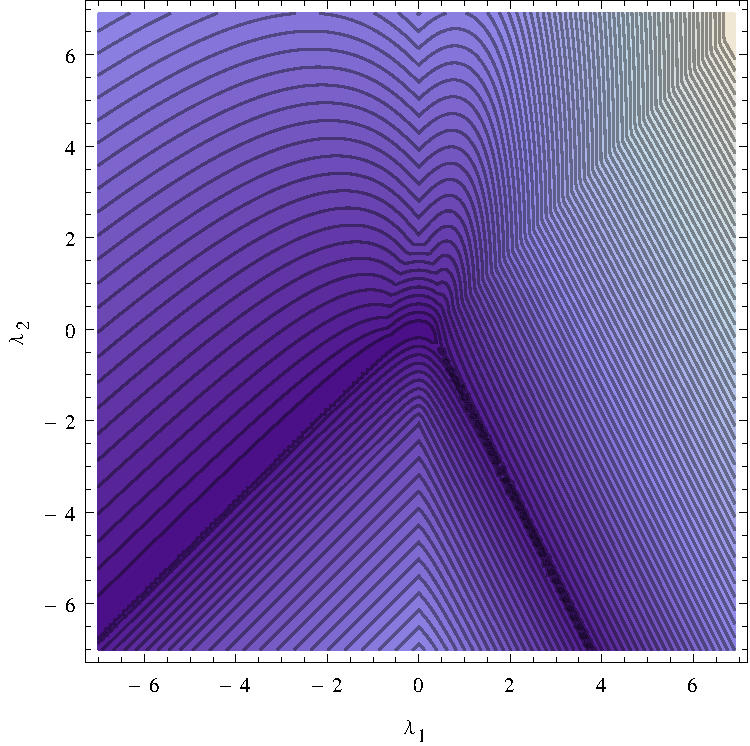
\includegraphics[scale=0.7]{Figures/hamgap.pdf}
\caption{{\em The plot shows the contour lines of the gap of the quantum Hamiltonian with \eqref{hamlimbs} switched on as a function of the two coupling co}}
\label{f1d}
\end{figure}
On the classical statistical frame instead the absence of phase transitions can be explained in terms of the failure of Peierls argument. The argument, in its most concise form, goes as follows. Consider one of the configurations $\{ \sigma \}$ of lowest energy, in which the spin variable $\sigma$ is the same on all the lattice sites. They will be of course the only relevant ones at zero temperature. As soon as the temperature is switched on one can ask which are the typical configurations characterizing the thermodynamics and whether ``magnetization'' is zero or not, in the therodynamic limit, for any nonzero value of the temperature. The first guess is to excite the ``ground state'' configuration placing an island of different numbers in the middle. Let $L$ be the length of the domain wall, then the free energy difference is given by
\be 
\Delta F = 2 L J - T \Delta S
\ee
Here is the keypoint: in the case of the Ising model the entropy difference is given understimating the number of this simple excited configurations with $2^L$, so that
\be \label{df}
\Delta F \le 2 L J - T \log 2^L = L ( 2 J - T \log 2 ) \le 0
\qquad \Rightarrow \qquad
T \ge \frac{2 J}{ \log 2 } \simeq T_c
\ee 
Thus the excited states becomes relevant only at a finite value of $T$. However in the coprime model \eqref{classham} the excited states are many more and their entropy difference with a ground state do not scale as the length $L$ of the domain wall, but as the area of the island inside the wall. Indeed let us consider the coprime statistical model with $q=5$. Pick up the ground state made up e.g. of $3$s. The latter can be excited with an island composed of all equal integers sharing no common divisors with $3$. However, since the coprime interaction makes no distinction between $2$ and $4$, there are $2^V$ possible excited states composed of all possible combinations of $2$ and $4$ (see Figure \ref{peierls}), where $V$ is the number of sites \emph{inside} the domain wall. Then for fixed length $L$ the entropy difference can be overstimated as
\be 
\Delta S \ge \log ( 2^L 2^V ) \underset{L \to \infty}{\sim} L^2 \log 2
\ee
Going back to \eqref{df} it is thus clear that the entropy contribution becomes dominant in the thermodynamic limit as soon as the temperature is switched on, the transition temperature $T_c$ shrinks to $0$ when the length of domain wall is sent to infinity and the model is always disordered.


\begin{figure}[H]
\hspace{-0.7cm}
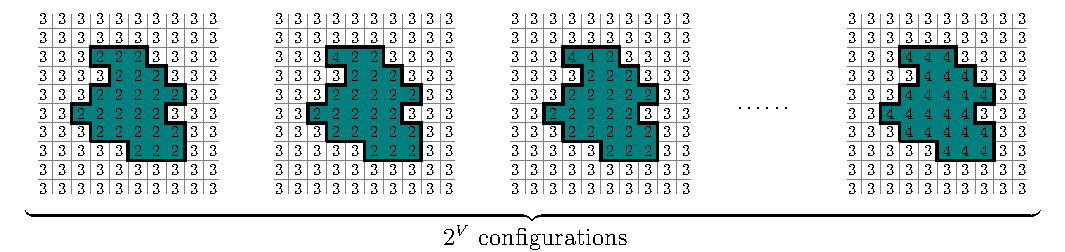
\includegraphics[scale=0.95]{Figures/peierls.pdf}
\caption{{\em For fixed length $L$ of the domain wall, there are $2^V$ possible configurations having the same energy difference with the ground state energy, being $V$ the number of cells inside the contour. Thus the number of states made of one Peierls island of length $L$ is always less than $2^V 2^L$, where $V \sim L^2$ in the limit $L \to \infty$. }}
\label{peierls}
\end{figure}

\noindent
The absence of phase transition on the 2d statistical model can be easly checked numerically by computing the specific heat as a function of the temperature $T$ 
\be 
c(T) = \frac{\partial \med{ \mathcal{H} } }{ \partial T } = \frac{ \med{ \mathcal{H}^2 } - \med{ \mathcal{H} } }{ T^2 }
\ee
The latter is easly obtained by sampling the Boltzmann distribution using a simple Metropolis algorithm \cite{metro} in which the move is to change randomly the integer on a random site. The presence of a critical point would be signaled by a spike in the graph of $c(T)$ for some value of $T$, representing a divergence of this function with some critical exponent $\alpha$. The results are shown in Figure \ref{specheat}. The specific heat per lattice site exhibits a maximum for a value of $\beta$ between $1$ and $2$, but no sign of divergences indicates the absence of a second order phase transition in this statistical model.

\begin{figure}[H]
\center
\makebox[0pt][c]{
\hspace{-10mm}
\begin{minipage}{0.52\textwidth}
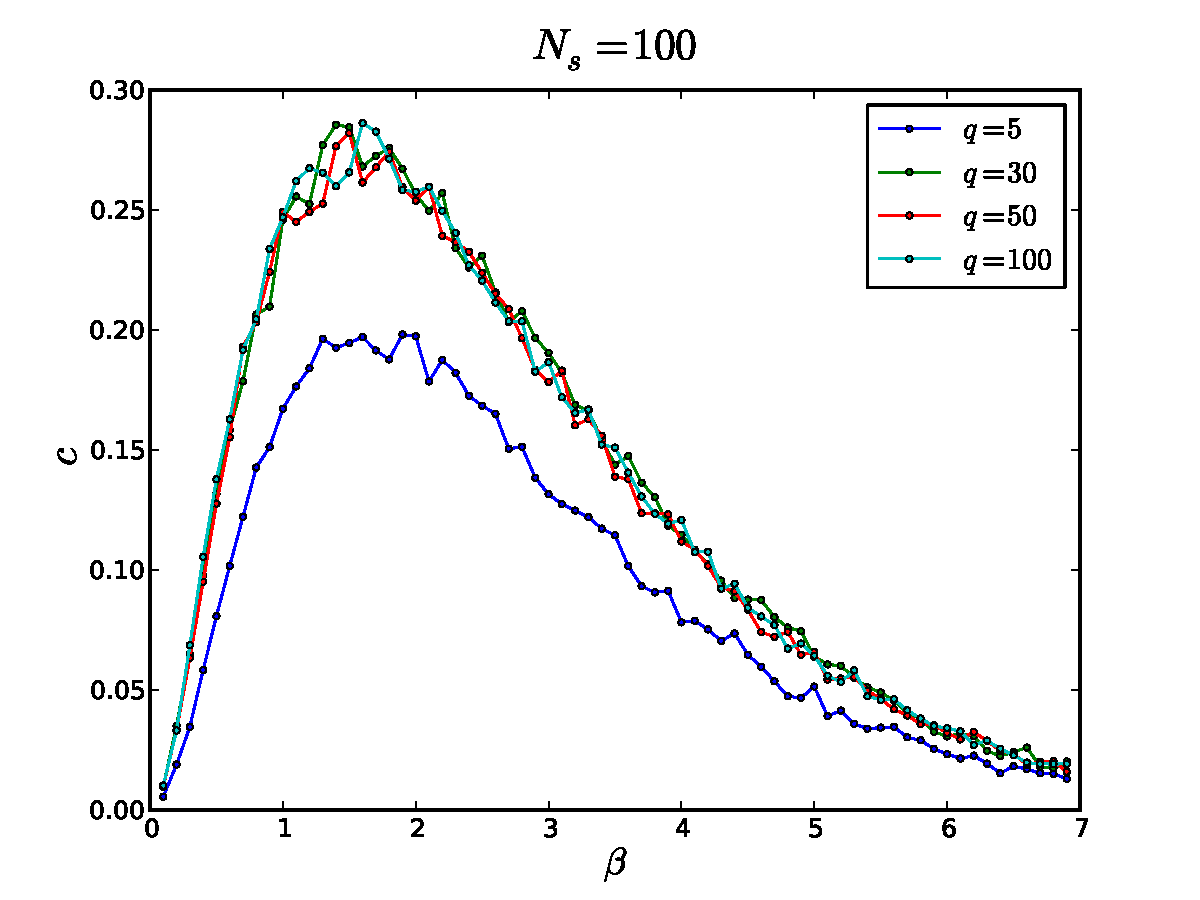
\includegraphics[scale=0.45]{Figures/spec.pdf}
\end{minipage}
\begin{minipage}{0.53\textwidth}
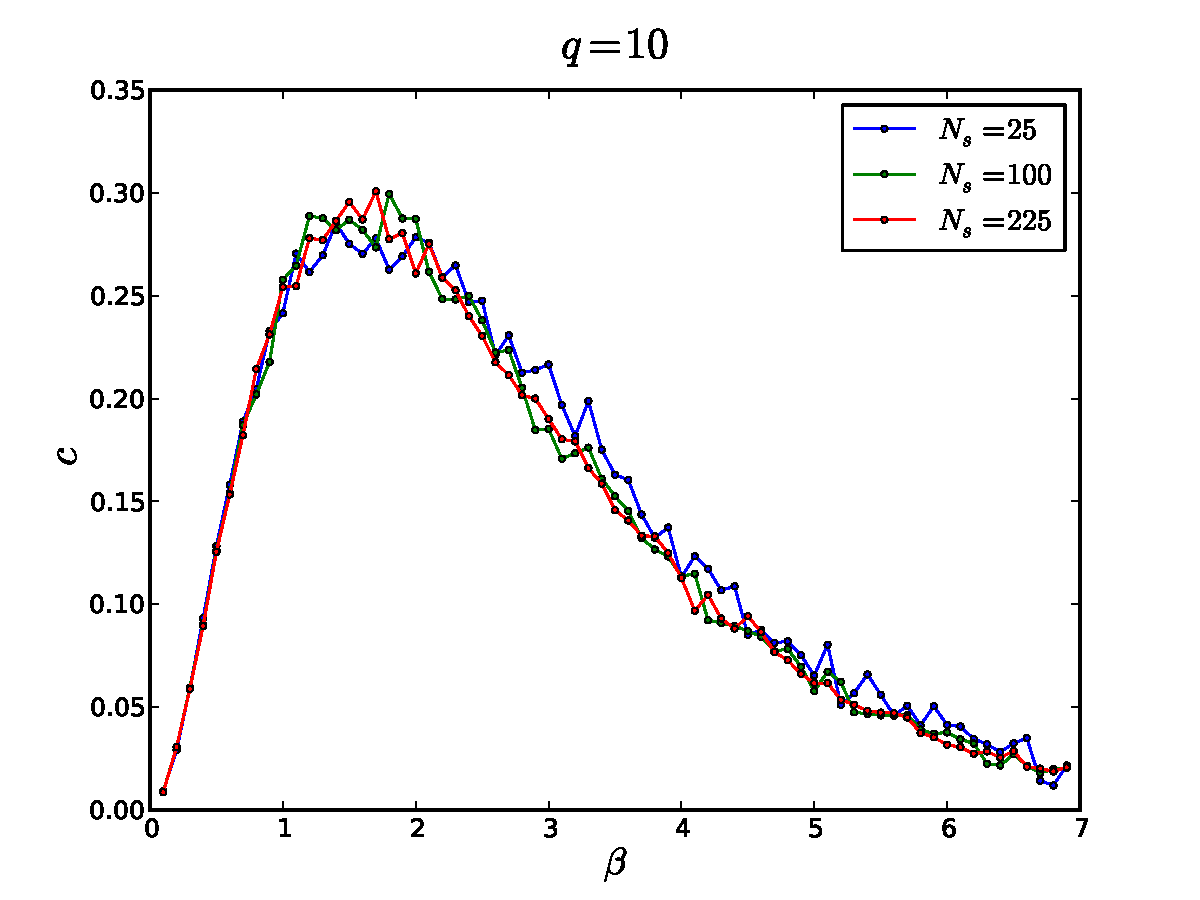
\includegraphics[scale=0.45]{Figures/scalspec.pdf}
\end{minipage}}
\caption{{\em In both plots the samples are taken from a single stocastic chain starting from a random configuration. The samples are taken after a Montecarlo time $t_{eq} = 10^4 \cdot N_s$, one each time interval of length $\Delta t = 600$, to ensure their independence. Here $N_s$ is the number of lattice sites. Each average necessary to compute the specific heat is performed over $3000$ realizations of the Boltzmann distribution. The plot on the left shows the specific heat per lattice site as a function of the inverse temperature $\beta$ for fixed $N_s$ and varying $q$, while the finite size scaling for fixed $q$ is shown on the right. The absence of a PT is evident from the analyticity of the numerical curve.     }}
\label{specheat}
\end{figure}
 
\vspace{1cm}
\begin{flushleft}\large
\textbf{Acknowledgements}
\end{flushleft}

We thanks xxx... 

\newpage
\appendix
\section{Basic elements of graph theory}\label{Appgraphtheory}

\section{Maximum degree}\label{Appmaxdegree}
It is possible to estimate the rate of growth with the number $q$ of the maximum degree of the graph based on the coprimality matrix $\widehat \Phi$. 
This estimate is based on the assumption of the statistical independence of the prime numbers and it goes as follows. Given a number $q$, 
let's first determine the maximum index $s$ such that the number made of the product of the first $s$ consecutive primes is less than $q$ 
\be 
\hat n \,=\, p_1 \times p_2 \ldots \times p_s \,< \, q \,\,\,.
\label{goodnumber}
\ee
Such number $\hat n$ is associated to one of the vertices with the maximum degree in the range $(2,q)$, this number divides 
all numbers multiples of $p_1 =2$, all those which are multiples of $p_2 = 3$, all those multiples of $p_3 = 5$, etc. Let's now estimate how many numbers 
have common factors with $\hat n$ using a probability argument. The total number of numbers that are divisible by $2$ is given by $q$ times the 
probability that a number is divisible by $2$, which is $\frac{1}{2}$, so $q \times \frac{1}{2}$. Those which are divisible by $3$ are given, naively, by 
$q \times \frac{1}{3}$. However among these multiples of $3$ we have to subtract those numbers that were already counted as divisible by $2$ (as, for instance, the number $6$). So the genuine numbers which are divisible by $3$ but not also by $2$ are given by $q$ multiplied for the probability $\hat p_3$ that a number is divisible by $3$ but not by $2$ 
\be 
\hat p_3 \,=\,\frac{1}{3} \, \left(1 - \frac{1}{2}\right) \,\,\,. 
\ee
Analogously, we can count the genuine numbers divisible by $5$ but not divisible for $2$ and $3$, in term of the corresponding probability 
\be 
\hat p_5 \,=\,\frac{1}{5} \,\left(1 - \frac{1}{2}\right) \, \left(1 - \frac{1}{3}\right) 
\ee 
and, more generally, 
\be 
\hat p_k \,=\,\frac{1}{p_k} \,\prod_{m=1}^{k-1} \left(1 - \frac{1}{p_m}\right) \,\,\,.
\ee
In this way, we predict that the maximum degree grows as 
\be 
d_{max} \,\sim\, q \, \sum_{k=1}^s \hat p_k \,\,\,.
\label{estmd}
\ee 
Notice that the number of terms included in the sum depends on the number $q$ itself: therefore there will be a sequence of discontinuities of the 
corresponding slope each time that $q$ overpass the values 
\be
2\, ,6 \,, 30\,, 210 \,, 2310 \,, 30030 \, \ldots 
\ee 
associated to the sequence of numbers $\hat n$.\\ Taking $q\rightarrow \infty$, which means $s \rightarrow \infty$, the ratio $d_\mathrm{max}/q$ is given by the infinite sum
\be \label{pseries}
\frac{d_\mathrm{max}}{q} \underset{ q \to \infty }{ \sim } \sum_{n=1}^\infty \,\frac{1}{p_n} \prod_{m=1}^{n-1} \left(1 - \frac{1}{p_m}\right)
\ee
The series is convergent since
\be \label{hseries}
\sum_{n=1}^\infty \,\frac{1}{p_n}  \exp \( \sum_{m=1}^{n-1} \left(1 - \frac{1}{p_m} \right) \) < \sum_{n=1}^\infty \,\frac{1}{p_n}  \exp \( - \sum_{m=1}^{n-1}  \frac{1}{p_m}  \) < \sum_{n=1}^\infty \,\frac{1}{p_n}  \frac{ e^{ \frac{\pi^2}{6} }}{ \log {p_n}  }
\ee 
where the last inequality follows from the fact that the truncated sum of the reciprocals of the primes is bounded by
\be 
\sum_{p < n } \frac{1}{p} > \log \log n - \log \frac{\pi^2}{ 6 } 
\ee
The series in the last member of \eqref{hseries} converges as a consequence of the prime number theorem, which states that the magnitude of the $n$-th prime number goes as
\be 
p_n \underset{ n \to \infty }{ \sim }  n \log n
\ee
so that the general term behaves asimptotically as
\be 
\frac{1}{ p_n \log p_n } \underset{ n \to \infty }{ \sim } \frac{1}{ n (\log n)^2 }
\ee
which is enough to make the series convergent.\\
However, since the maximum degree of a graph cannot exceed the number of vertices of the graph, \eqref{pseries} must give a result smaller than $1$. This has to hold if the assumption leading to \eqref{pseries} is correct, namely that the position of the $n$-th prime number is independent from the positions of the others.\\
In fact the result is exactly $1$, as the truncation of \eqref{pseries} can be put in the telescopic form
\begin{align*}
\sum_{n=1}^N \, \(1 - 1 + \frac{1}{p_n} \) \prod_{m=1}^{n-1} \left(1 - \frac{1}{p_m}\right)  & = 
\sum_{n=1}^N {} \prod_{m=1}^{n-1} \left(1 - \frac{1}{p_m}\right) - \sum_{n=2}^{N+1} {} \prod_{m=1}^{n-1} \left(1 - \frac{1}{p_m}\right)  =  \\[1mm]
& =  1 - \prod_{m=1}^{N} \left(1 - \frac{1}{p_m}\right)  \quad \underset{ N \to \infty }{  \rightarrow } \quad  1  - \frac{1}{ \zeta(1) } = 1 
\end{align*}
where
\be 
\zeta(z) = \prod_{k=0}^{\infty} \(1 - p_k^{-z} \)^{-1}
\ee
is the product representation of the Riemann Zeta function, whose only pole is $z=1$.

\newpage

\begin{thebibliography}{1}
\bibitem{ccee} J. L. Cardy, P. Calabrese, \emph{Entanglement Entropy and Quantum Field Theory}, J. Stat. Mech. (2004)
\bibitem{kogut} J. B. Kogut, \emph{An introduction to lattice gauge theory and spin systems}, Rev. Mod. Phys. 51, 659 (1979)
\bibitem{metro} N. Metropolis, A. W. Rosenbluth, M. N. Rosenbluth, A. H. Teller, E. Teller, \emph{Equations of State Calculations by Fast Computing Machines}, J. Chem. Phys. 21 (6), 1087–1092 (1953)
\bibitem{bpz} A.A. Belavin, A.M. Polyakov, A.B. Zamolodchikov, \emph{Infinite conformal symmetry in two-dimensional quantum field theory}, Nucl. Phys. B 241, 333 (1984)
\bibitem{sachdev} S. Sachdev, \emph{Quantum phase transitions}, Cambridge University Press (2011)
\bibitem{bcn}  H. W. J. Bl\"ote, J. L. Cardy, M. P. Nightingale, \emph{Conformal Invariance, the Central Charge, and Universal Finite-Size Amplitudes at Criticality}, Phys. Rev. Lett. 56, 742 (1986)

\bibitem{dots} Vl. S. Dotstenko, \emph{Critical behaviour and associated conformal algebra of the $Z_3$ Potts model}, Nucl. Phys. B. 235, 54 (1984)
\bibitem{aff} I. Affleck, \emph{Universal term in the free energy at a critical point and the conformal anomaly}, Phys. Rev. Lett. 56, 746 (1986)
\end{thebibliography}

\end{document}

